% !TEX root = ../thesis-example.tex
%
\chapter{Représentations visuelles}
\label{ch:visual_representation}

\cleanchapterquote{Ces petits morceaux d’espace visuel,\\
dont la connexion n’est pas donnée d’avance,\\
par quoi voulez-vous qu’ils soient connectés,\\
sinon par la main?}{Gilles Deleuze}
{\textit{Qu'est ce que l'acte de création?}\\
conférence donnée à la FEMIS \cite{deleuze_deux_2003}}

\vspace*{\fill}

%TODO : résumé\\
%voir mp.TUI.key pour les images à inclure

\noindent Divers facteurs contribuent à l'aspect visuel des instruments de musique, et y joue un rôle esthétique mais également fonctionnel, notamment en tant qu'ils contribuent à y définir la topologie de l'interaction. Nous avons vu dans les chapitres précédents que les \glspl{DMI} intègrent des fonctions liées à l'interprétation du geste, à la production du son, à la composition musicale ainsi qu'à l'utilisation de toute sorte de modèles intermédiaires pour le design de l'interaction. Chacun de ces aspects hérite de représentations qui leur sont attachées: représentations du son (temporelles, fréquentielles, intensités de paramètres audio, etc.), représentations musicales (le vaste héritage de la notation musicale traditionnelle), auquel s'ajoute potentiellement tout le langage du design graphique.\\
\indent Dans les \glspl{DMI}, la possibilité d'afficher des éléments graphiques de manière dynamique sur un moniteur, mais également d'interagir directement avec ces éléments quand le moniteur est tactile, laisse envisager un vaste terrain où peuvent s'entrecroiser diverses représentations liées aux aspects susmentionnés dans des composites hybrides. L'interaction sur ces objets graphiques est elle-même un champ d'exploration ouvert dans lequel les interactions traditionnelles héritées de la bureautique s'avèrent très vite insuffisantes.\\
\indent Après une étude de ces différents aspects, je présenterai la librairie mp.TUI, dont le développement illustre l'effort entrepris dans cette perspective, ainsi qu'une application pratique de l'utilisation du protocole MP décrit au chapitre précédent.

\clearpage

%%%%%%%%%%%%%%%%%%%%%%%%%%%%%%%%%%
\section{Aspects visuels du design d'instrument}

\noindent La conception d'un instrument englobe plusieurs aspects qui affectent son allure visuelle. Je passerai ici en revue quelques-uns de ces aspects, en m'appuyant notamment sur des exemples d'instruments acoustiques, pour souligner certaines continuités avec les développements entrepris ici dans le domaine numérique.

\subsection{Adaptation à la production du son}

%\todo{éliminer les redites du chapitre hardware}

\noindent L'apparence des instruments est en partie définie par la recherche d'une certaine qualité de son. Bien que cela soit particulièrement évident pour les instruments acoustiques dont les formes ont des conséquences directes sur le rendement sonore (cf. exemple figure \ref{fig:visual_representation:fhole}), les profils particuliers issues de la lutherie traditionnelle ont également donné naissance à un certain nombre d'éléments iconiques (par exemple, les ouïes du violons ou les touches noires et blanches du piano) et de facteurs de forme (par exemple, une taille plus grande produit un son plus grave) associés à l'idée d'un instrument, comme le rappelle Trevor Pinch dans son interview de Robert Moog \cite{pinch_why_2001}: \iquote{Les claviers étaient toujours là, et chaque fois que quelqu'un voulait prendre une photo, pour une raison ou une autre, c'était mieux si on jouait du clavier. Les gens comprennent alors vous faîtes de la musique. (...) Cette pose [prenant la pose, bras gauche tendu tandis que la main droite joue du clavier] associe graphiquement la musique et la technologie.}\footnote{``The keyboards were always there, and whenever someone wanted to take a picture, for some reason or other it looks good if you’re playing a keyboard. People understand that then you’re making music. (...) This pose here [acts out the pose of the left arm extended while the right hand plays a keyboard] graphically ties in the music and the technology.''}.\\
\indent De plus, les \glspl{DMI} peuvent intégrer des transducteurs acoustiques, tels que des microphones piézoélectriques ou des haut-parleurs tactiles (comme nous l'avons vu à la section \ref{sec:interfaces:part_acoustique}), qui influencent la conception acoustique de leurs composants matériels et donc les facteurs de forme évoqués précédemment.

%------------ Figure : f-hole et boehm -----------
\begin{figure}[!htbp]
	\captionsetup{format=plain}%
	\centering
	\begin{minipage}[t]{0.48\textwidth}
		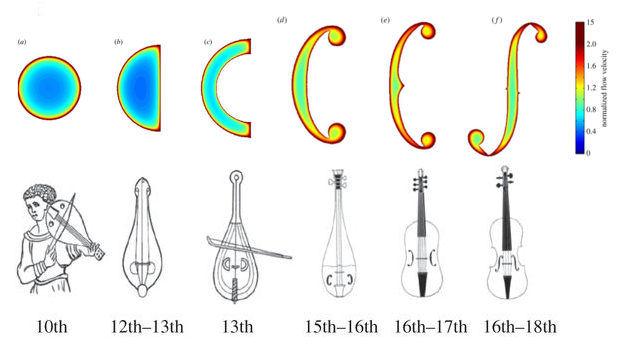
\includegraphics[width=\linewidth]{gfx/06_visual_representation/f-hole.png}
		\caption[Évolution de la forme des ouïes du violon et influence sur la projection acoustique]{Évolution de la forme des ouïes du violon et influence sur la projection acoustique, d'après \cite{nia_evolution_2015}}
		\label{fig:visual_representation:fhole}
	\end{minipage}
	\hspace{.02\linewidth}
	\begin{minipage}[t]{0.48\textwidth}
	    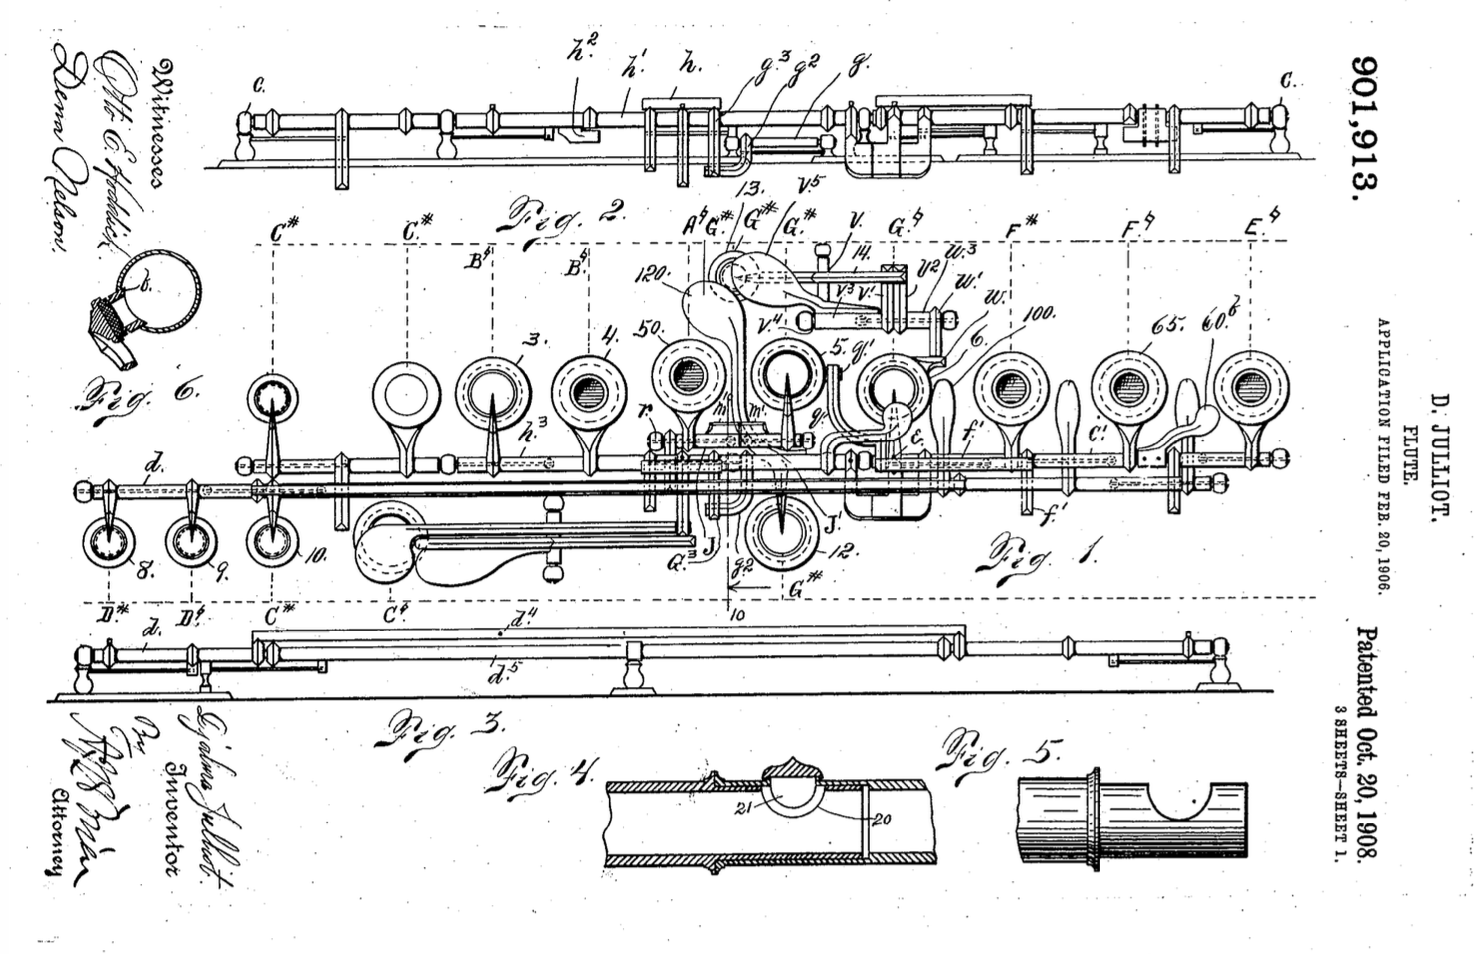
\includegraphics[width=\linewidth]{gfx/06_visual_representation/Julliot_patent.png}
		\caption[Brevet sur l'amélioration du clétage des flûtes de Boehm]{Extrait du brevet de J. Djalma sur \iquote{l'amélioration du clétage des flûtes de Boehm}, 1908.}
		\label{fig:visual_representation:boehm}
	\end{minipage}
\end{figure}


\subsection{Adaptations ergonomiques}

%\todo{éliminer les redites du chapitre algorithms}

\noindent L'instrument s'adapte également au corps. Un exemple intéressant est l'évolution du traverso vers la flûte de concert occidentale, à l'aide du système Boehm dans les années 1840 (cf. figure \ref{fig:visual_representation:boehm}). Ce système de clétage découple la topologie gestuelle de la topologie du flux d'air et de la topologie de résonance. En utilisant des manches et des platines, il permet d'accroître la puissance sonore par l'élargissement des trous et leur déplacement à des endroits adéquats pour la résonance, tandis que les touches peuvent être placées à des endroits adaptés à la position des doigts du flûtiste.\\
\indent Le système Boehm peut être qualifié de ``modèle intermédiaire'' entre le geste et la production sonore, fait d'un système mécanique dans ce cas. La plupart des instruments combinent divers ``modèles intermédiaires'' pour amplifier, enrichir, déplacer, focaliser, multiplier les gestes des interprètes et générer des mouvements hors du champ des possibilités du corps humain : pédales de grosse caisse, marteaux et amortisseurs pour piano, archets et plectres, etc.

\subsection{Représentations liées à la théorie musicale}
\label{ch:visual_representation:music-theory}

%------------ Figure : keyboard et TUI - scale -----------
\begin{figure}[!htbp]
	\captionsetup{format=plain}%
	\centering
	\begin{minipage}[t]{0.48\textwidth}
		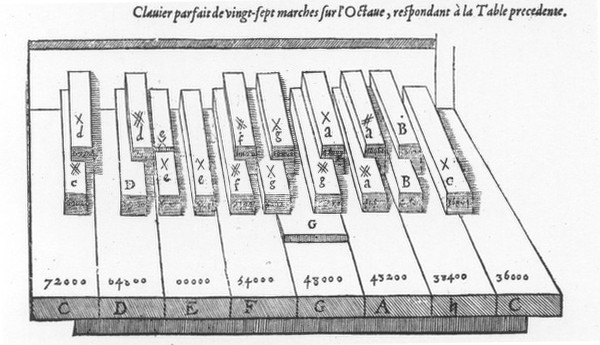
\includegraphics[width=\linewidth]{gfx/06_visual_representation/Mersenne_clavier.png}
		\caption[Clavier à 27 touches de Mersenne]{Le ``clavier parfait de vingt-sept marches sur l'Octave' de Mersenne (1636)}
		\label{fig:visual_representation:MersenneKeyboard}
	\end{minipage}
	\hspace{.02\linewidth}
	\begin{minipage}[t]{0.48\textwidth}
	    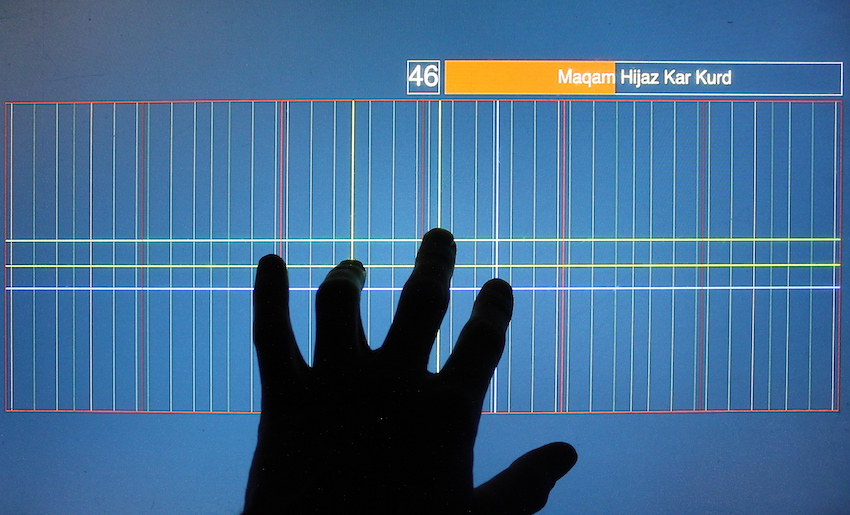
\includegraphics[width=\linewidth]{gfx/06_visual_representation/mpTUI_pitchgrid_72dpi.png}
		\caption[Grille de hauteur micro-tonale dans mp.TUI]{Une grille de hauteur avec une représentation micro-tonale réalisée avec mp.TUI. La luminosité des lignes verticales varie en fonction de la quantité de quantification.}
		\label{fig:visual_representation:pitch_grid}
	\end{minipage}
\end{figure}

\noindent Les instruments de musique intègrent également des éléments de théorie musicale. Par exemple, la partie supérieure d'un clavier (touches noires et blanches) représente la gamme chromatique, tandis que la partie inférieure (touches blanches seulement) représente la gamme diatonique de Do majeur. Le dimensionnement et le positionnement de ces touches est un compromis intéressant entre les contraintes mécaniques du système de marteaux et une représentation uniforme des échelles diatonique et chromatique. De plus, la largeur de l'octave est telle qu'elle tient sous une main tendue et vient réifier dans l'instrument la notion d'équivalence des octaves, en permettant de jouer n'importe quel intervalle à l'intérieur d'une octave avec une seule main. Les claviers ont par ailleurs fait l'objet de nombreux développements expérimentaux\footnote{Voir notamment \cite{haury_petite_1999} pour un historique du clavier.} avec des dispositions de notes utilisant des grilles hexagonales ou plusieurs couches de touches (figure \ref{fig:visual_representation:MersenneKeyboard}) pour permettre le jeu dans des systèmes d'intervalles micro-tonaux.\\
\indent En tant que système symbolique, la théorie musicale peut être facilement encodée dans les ordinateurs. Les logiciels de production musicale contiennent tellement de fonctions et de règles basées sur la théorie musicale qu'il serait difficile de toutes les représenter sur l'interface. Thor Magnusson parle ainsi ``d'outils épistémiques'' pour décrire les \glspl{DMI}, affirmant qu'il sont conçus avec ``un tel degré de pertinence symbolique qu'ils deviennent un système de connaissance et de pensée dans leurs propres termes'' \cite{magnusson_epistemic_2009}. Pour le \textit{musicien numérique}, ce ``système de connaissances'' est un paysage imaginaire à explorer, un territoire sonore pour lequel l'interface de l'instrument peut métaphoriquement prendre le rôle d'une carte géographique, ou d'un cockpit de pilote \cite{vertegaal_towards_1996}.

\subsection{Représentations liées au contexte de performance}

\noindent Si l'on considère les instruments de musique comme des ``instruments pour musiquer'' en reprenant la définition de Christopher Small (cf. p. \pageref{def:musicking}), alors les partitions, les salles de concert, le public et plus généralement, le contexte de la performance influencent aussi la conception et la représentation des instruments. Les partitions orientées (figure \ref{fig:visual_representation:table_music}) sont un exemple d'adaptation de la partition au contexte de la ``musique de table'', permettant dans ce cas aux musiciens de lire une même partition lorsqu'ils sont assis autour d'une table. De même, les \glspl{DMI} collectifs (cf. \ref{sec:ephemeral:origins:collectiveDMIs}) peuvent adapter leur représentation au nombre d'interprètes en présentant à chacun d'eux un groupe d'éléments d'interface utilisateur orientés vers eux (figure \ref{fig:visual_representation:multi_orientation}).\\
\indent Comme exemples de l'influence du lieu de concert sur le design visuel de l'instrument, on peut notamment évoquer les modélisations de l'espace acoustique du lieu pour venir contrôler la spatialisation du son (cf. figure \ref{fig:visual_representation:spat}) ou --~à l'inverse~-- la projection sur le lieu d'un \textit{mapping vidéo} en correspondance avec la musique\footnote{ou une ``musique visuelle'' comme l'appelle Serge de Laubier} (cf. \ref{fig:visual_representation:pucemuse-monument}).

%------------ Figure : keyboard et TUI - scale -----------
\begin{figure}[!htbp]
	\captionsetup{format=plain}%
	\centering
	\begin{minipage}[t]{0.48\textwidth}
		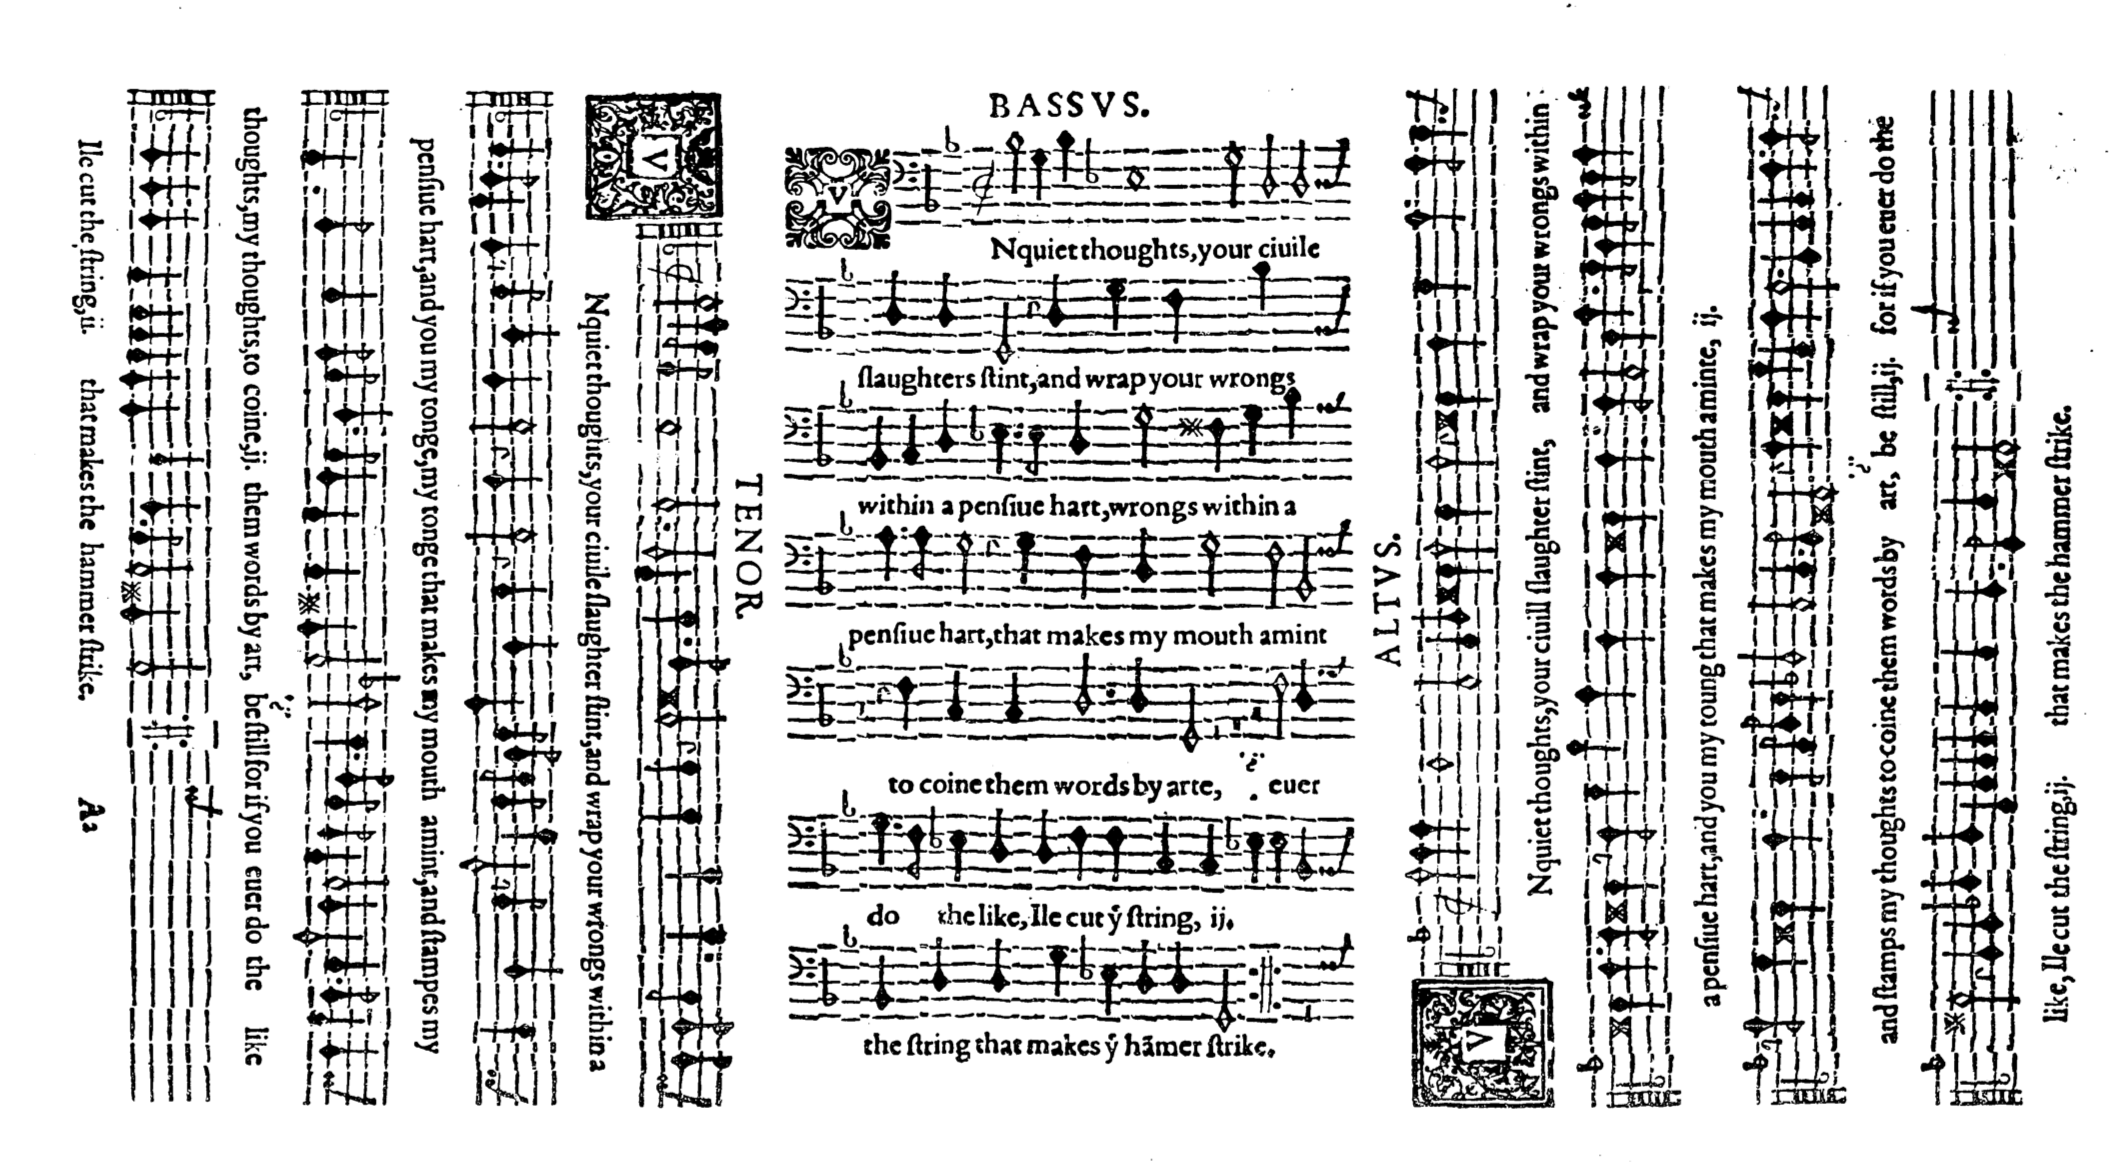
\includegraphics[width=\linewidth]{gfx/06_visual_representation/Dowland-firstBookOfSonges.png}
		\caption[Partition ``de table'' à plusieurs voix]{Partition ``de table'' à plusieurs voix (John Dowland - First Booke of Songes or Ayres. Édition Peter Short, London, 1597)}
		\label{fig:visual_representation:table_music}
	\end{minipage}
	\hspace{.02\linewidth}
	\begin{minipage}[t]{0.48\textwidth}
	    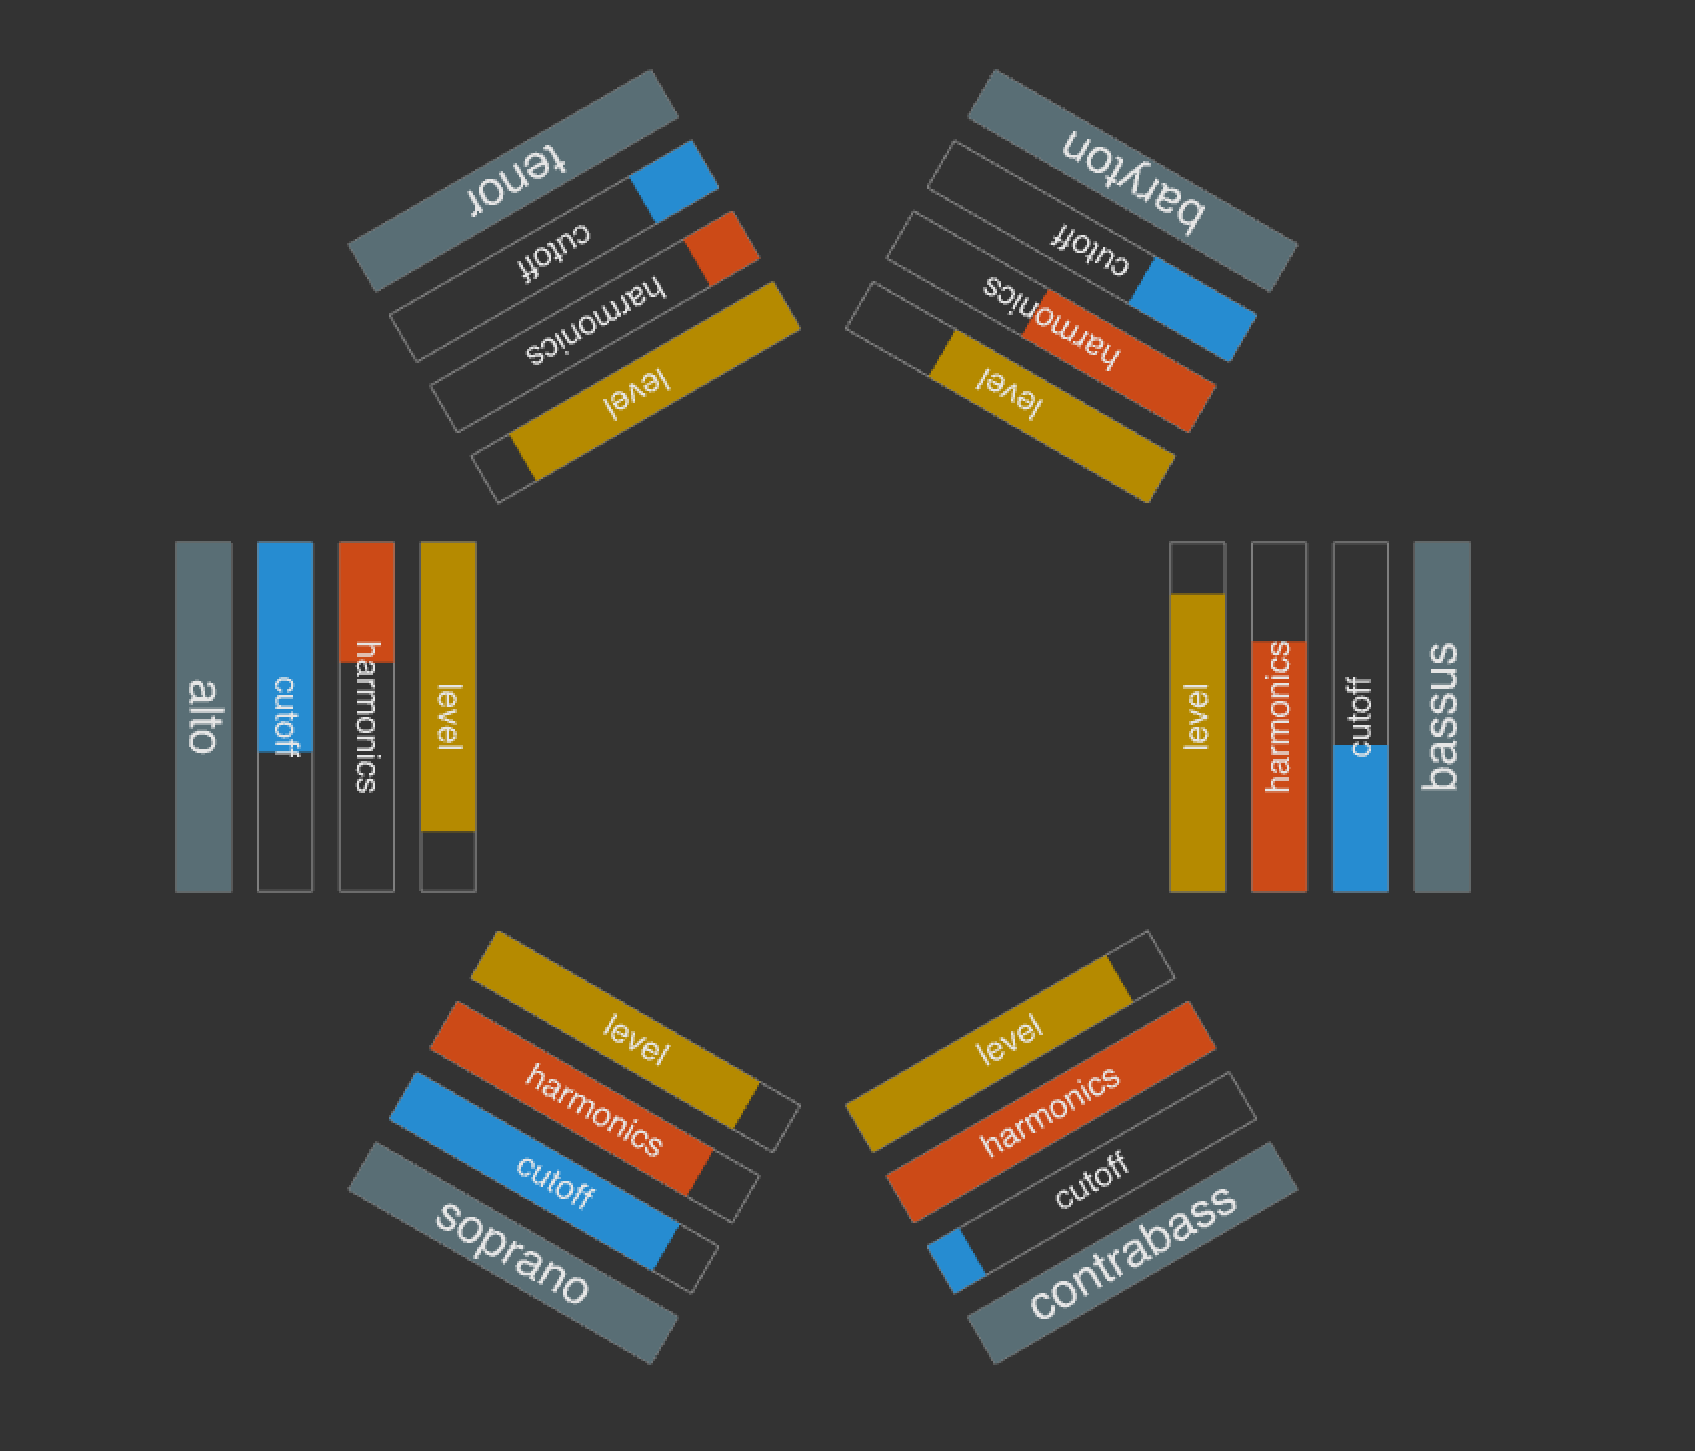
\includegraphics[width=\linewidth]{gfx/06_visual_representation/mpTUI_multi-orientation.png}
		\caption[Interface visuelle adaptée pour 6 joueurs]{Interface visuelle adaptée pour 6 joueurs situés autour d'une interface de jeu commune, réalisée avec la librairie mp.TUI.}
		\label{fig:visual_representation:multi_orientation}
	\end{minipage}
\end{figure}
%------------ Figure : keyboard et TUI - scale -----------
\index[people]{dowland@Dowland, John!firstbookofsonges@\textit{First Booke of Songes or Ayres}}

%------------ Figure : spat et PM -----------
\begin{figure}[!htbp]
	\captionsetup{format=plain}%
	\centering
	\begin{minipage}[t]{0.48\textwidth}
		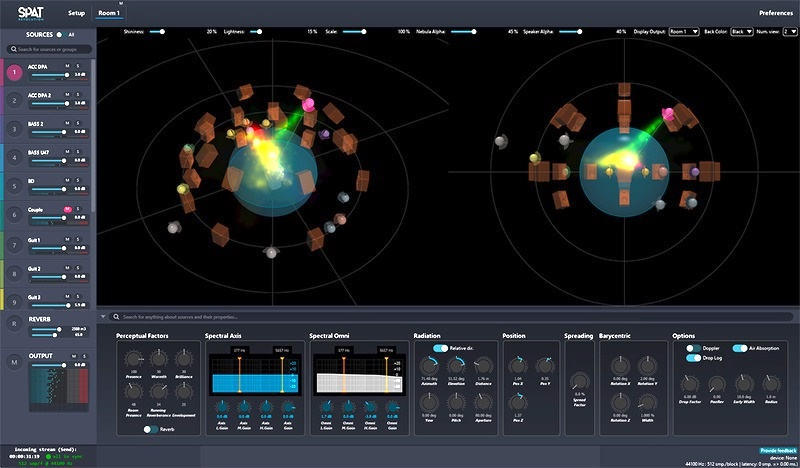
\includegraphics[width=\linewidth]{gfx/06_visual_representation/IRCAM-spat.jpg}
		\caption[IRCAM Spat Revolution]{L'interface du logiciel ``Spat Revolution'' de l'IRCAM modélise l'espace de projection acoustique du lieu de concert.}
		\label{fig:visual_representation:spat}
	\end{minipage}
	\hspace{.02\linewidth}
	\begin{minipage}[t]{0.48\textwidth}
	    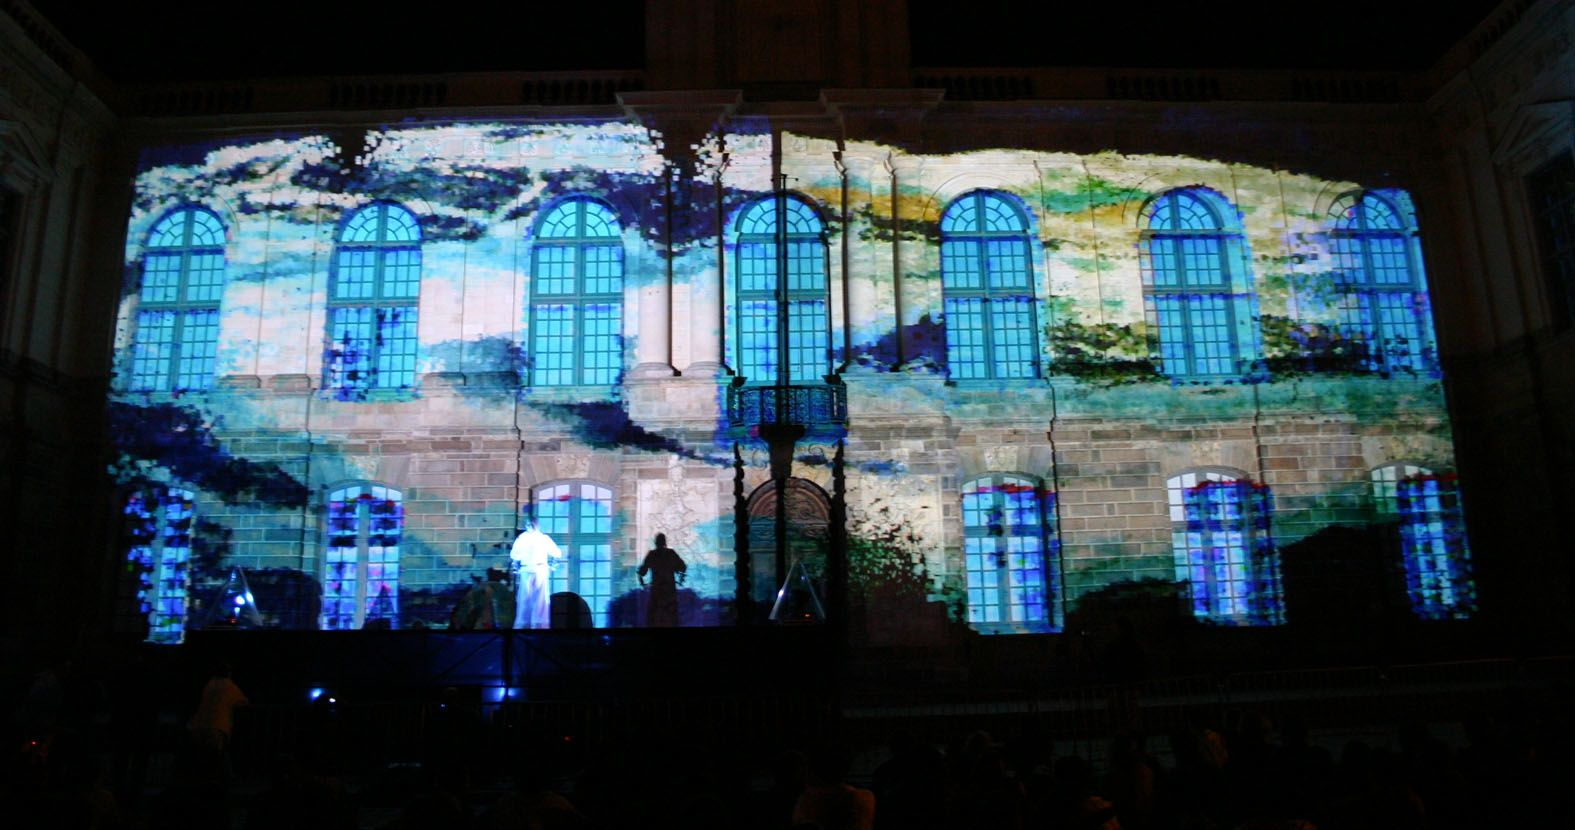
\includegraphics[width=\linewidth]{gfx/06_visual_representation/PuceMuse-Facade.jpg}
		\caption[Projection monumentale, Puce Muse]{Projections monumentales de ``musique visuelle'', controlée de manière synchrone à la ``musique sonore''. Photographie © Puce Muse.}
		\label{fig:visual_representation:pucemuse-monument}
	\end{minipage}
\end{figure}
%------------ Figure : spat et PM -----------
\index[people]{delaubier@De Laubier, Serge!traverse@\textit{Traverse de façade}}

\subsection{Représentations liées à l'expérimentation}

\noindent Le processus de conception des instruments de musique contient une grande part de travail empirique. Dans les \glspl{DMI}, l'ajustement des paramètres requiert une rétroaction sonore et visuelle directe pour affiner les réglages à la main, jusqu'à ce que l'instrument sonne et se prête au jeu. La représentation visuelle des réglages, sous la forme de potentiomètres, de sliders, ou d'autres éléments graphiques joue un rôle crucial et renseigne de manière beaucoup plus rapide qu'un affichage numériques, en offrant une appréciation relative et globale différents réglages (figure \ref{fig:visual_representation:numbers-vs-sliders}).\\
\indent C'est notamment pour cette raison que la ``programmation visuelle'' est un paradigme courant dans les environnements de lutherie numérique, tels que Max, PureData, Reaktor, etc. Non seulement elle est adaptée au paradigme de \textit{dataflow} que la programmation audio temps-réel adopte souvent, mais elle s'apparente également à une pratique de l'ingénierie audio basée le \textit{patching}, en même temps qu'elle offre une visualisation qui se prête à la manipulation directe.

%-------------------------- Figure : Numbers Vs Sliders ------------------------
\begin{figure}[!htbp]
	\captionsetup{format=plain}%
	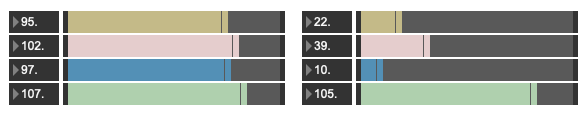
\includegraphics[width=\textwidth]{gfx/06_visual_representation/NumbersVsSliders.png}
	\caption[Représentation numérique et visuelle des paramètres]{La représentation visuelle des paramètres offre un aperçu plus rapide de leur valeur relative que leur représentation numérique.}
	\label{fig:visual_representation:numbers-vs-sliders}
\end{figure}
%-------------------------- Figure : Numbers Vs Sliders ------------------------

\subsection{Aspects esthétiques : l'instrument œuvre d'art}

\noindent Le design de l'interface visuelle de l'instrument se résume rarement à ses aspects fonctionnels. Les instruments de musique sont souvent l'œuvre d'un artisanat très pointu, voire des objets d'art. La finesse des détails et le souci de leur aspect esthétique jouent ainsi une part éminente dans le design final. Dans les interfaces visuelles des logiciels audio, on retrouve souvent ce soin esthétique, que cela soit sous forme d'un skeuomorphisme\footnote{le terme de skeuomorphisme est utilisé pour définir un élément de design dont la forme n'est pas directement liée à la fonction, mais qui reproduit de manière ornementale un élément qui était nécessaire dans l'objet d'origine.} (figure \ref{fig:visual_representation:skeuomorphisme}) cherchant à imiter le bois des instruments acoustiques, le métal et l'aspect physique des boutons sur les équipements hardware, ou d'un design plus épuré\footnote{sur les connexions entre le design d'interfaces et les arts graphiques, voir également les étonnants résultats obtenus en appliquant des modèles AI pour créer une interface à partir d'images photographiques dans \cite{troyer_mondrian_2019}.}  (figure \ref{fig:visual_representation:apparatum}).

%------------ Figure : skeuomorphisme et soin du design -----------
\begin{figure}[!htbp]
	\captionsetup{format=plain}%
	\centering
	\begin{minipage}[t]{0.48\textwidth}
		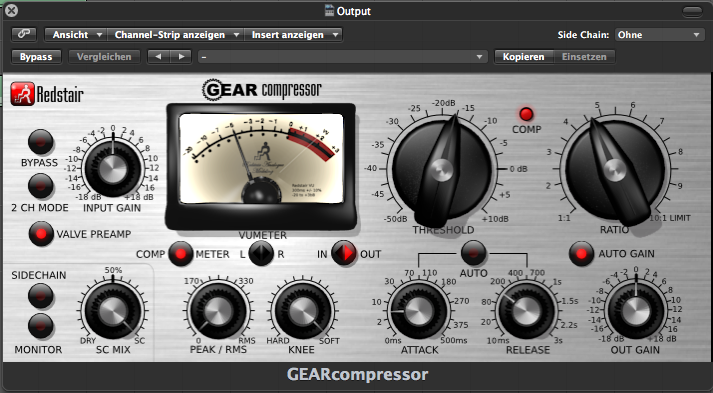
\includegraphics[width=\linewidth]{gfx/06_visual_representation/Redstair_GEARcompressor.png}
		\caption[Skeuomorphisme dans les logiciels audio]{Le skeuomorphisme dans les logiciels audio témoigne de l'importance accordée à l'esthétique, au-delà des fonctionnalités de l'interface. Photographie Klaus Göttling.}
		\label{fig:visual_representation:skeuomorphisme}
	\end{minipage}
	\hspace{.02\linewidth}
	\begin{minipage}[t]{0.48\textwidth}
	    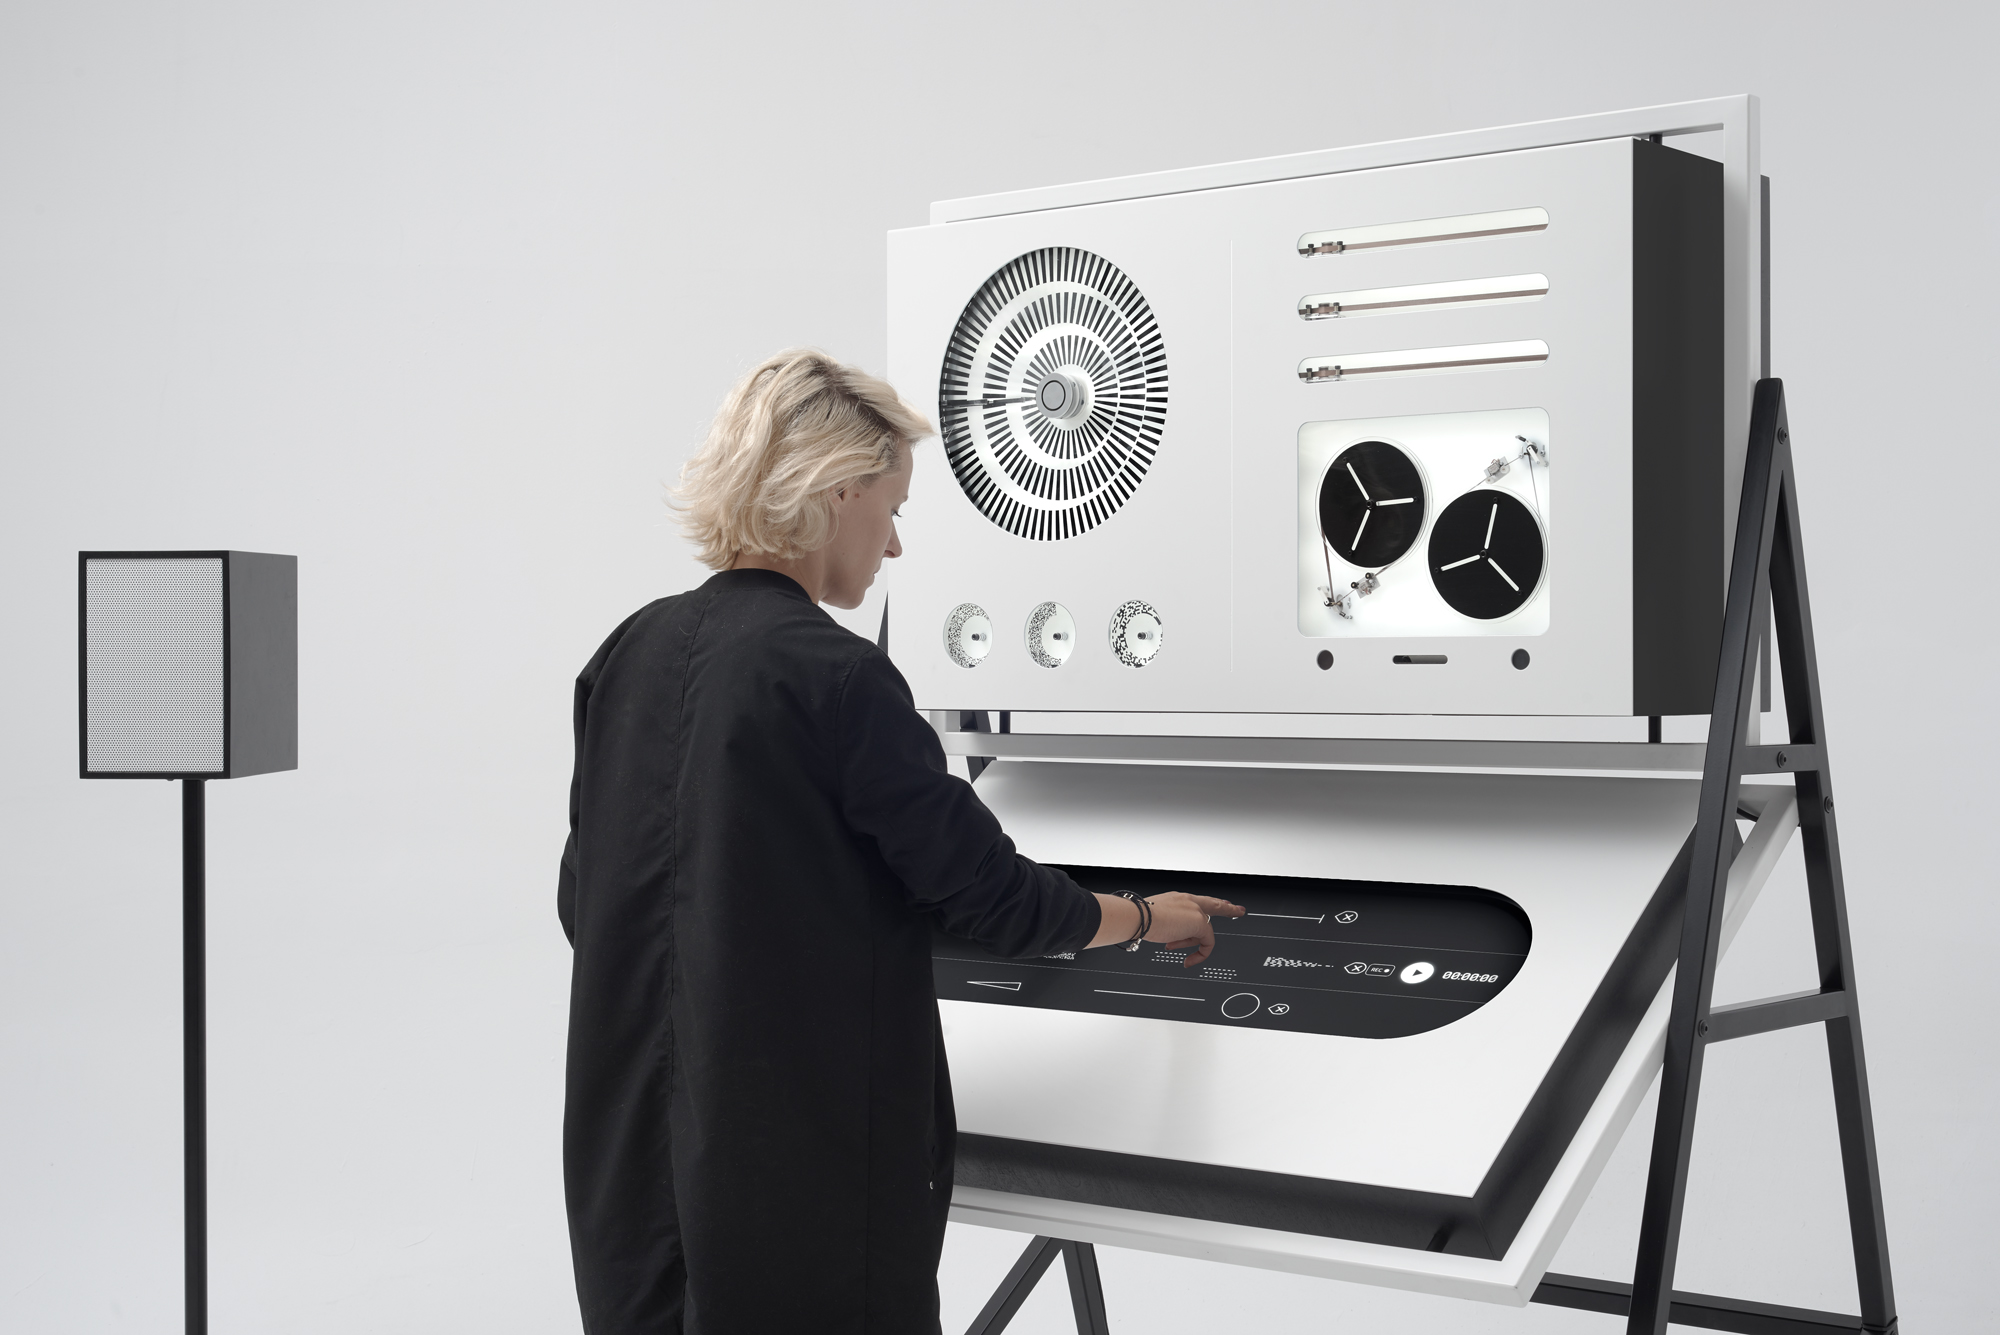
\includegraphics[width=\linewidth]{gfx/06_visual_representation/2018_06_26_PAN_GENERATOR_APPARATUM0396.jpg}
		\caption[Apparatum, par PanGenerator]{Le design minimal et soigné de l'instrument Apparatum. © panGenerator}
		\label{fig:visual_representation:apparatum}
	\end{minipage}
\end{figure}
\index[people]{pangenerator@PanGenerator (groupe)!apparatum@\textit{Apparatum}}

%------------ Figure : skeuomorphisme et soin du design -----------
%  TODO : amémiorer ce paragraphe
\noindent En tant qu'élément scénographique, la représentation visuelle joue un rôle essentiel dans l'esthétique et la poésie de l'instrument. Par exemple, dans la performance \textit{FIB\_R}\index[people]{forages@FORAGES (groupe)!fibr@\textit{FIB\_R}} : toute la performance visuelle video-projetée sur l'écran visible du public correspond à ce que les instrumentistes ont face à eux sur leur tablette. Le design de l'interface graphique est donc autant motivé par des aspects fonctionnels d'interaction, que des aspects esthétiques et poétiques.


%%%%%%%%%%%%%%%%%%%%%%%%%%%%%%%%%%%%%%%%%
\section{L'écran comme interface de jeu}

\subsection{L'écran, cockpit du musicien?}

\noindent En tant qu'\textit{outils épistémiques}, les \glspl{DMI} mettent en jeu un nombre extrêmement élevé de flux de données et de processus qui interagissent entre eux et avec l'interface. La représentation visuelle peut faciliter le \textit{monitoring} du bon fonctionnement de ces processus\footnote{Ce monitoring s'avère nécessaire lors de l'élaboration d'un instrument, mais aussi durant sa pratique, quand la mémoire fait défaut, ou que l'instrument instable est sujet à des dysfonctionnements.}, de leurs dynamiques, et la sélection de réglages dans des banques de données (presets, samples, etc.).

\subsubsection{Espace infini et savoir cartographique} 

\noindent L'écran donne en effet accès à un espace virtuellement infini, grâce à des systèmes d'onglets, de fenêtres multiples, de menus condensant différentes options, de zoom et déplacement sur des zones d'intérêt. L'exploration y est autant possible ``horizontalement'', c'est-à-dire parmi les différents éléments d'un même niveau de complexité, que ``verticalement'', c'est-à-dire dans la profondeur des différentes couches d'un même élément.\\
\indent Ce vaste territoire possède ainsi sa géographie et ses ``moyens de transport''. Si l'exploration peut se faire horizontalement (de manière ``touristique'', en parcourant les divers processus à disposition) ou en profondeur (de manière ``spéléologique'', en plongeant dans les entrailles d'un processus), elle peut aussi se faire par ``télé-transportation'': un preset peut rappeler une configuration complète correspondant à un terrain de jeu totalement différent.\\
\indent À mesure que les données emmagasinables sur les ordinateurs augmentent --~et plus encore, sur le net en tant qu'il constitue une excroissance de l'instrument numérique~-- la fonction de cartographie et de recherche de l'information utile prend de plus en plus d'importance. On peut en observer les signes dans la généralisation de l'intégration de moteurs de recherche dans les logiciels, notamment audio. Le numérique fait évoluer notre rapport aux outils d'une posture consistant à ``savoir le contenu'' à une posture consistant à ``savoir que ce contenu existe et comment le trouver''\footnote{\iquote{(...) my students tell me, the biggest problem they have in music production is finding their samples on their hard drive. They say ``I have so many kick drums on my Drive, that I've downloaded from so many places, that I can never find the one I want''. (...) now maybe it means that you don't need Stradivarius, you need a database programmer, that the most important thing in your life would be like, a really brilliant database that would allow you to intuitively retrieve whatever sample you wanted... In other words, that's in such a different domain but it may be, as I say, the single most important thing for a composer working today.} Nicolas Collins, cf. annexe \ref{appendix:collins}.}.\\
\indent Cependant, l'action de rechercher un contenu n'est pas \textit{a priori} un geste expressif. La conception d'un \gls{DMI} pour la performance passe ainsi par la circonscription d'un territoire dans lequel l'interaction soit suffisamment directe et intuitive pour que le musicien n'ait pas à réfléchir à la manière de se rendre à l'endroit désiré\footnote{\iquote{(...) it's a difficult thing to articulate but I think that if you give somebody too many choices of things to do, it will not be an expressive musical instrument because there's gonna be too much thinking (...) you have to sort of find a spot in between} Nicolas Collins, cf. annexe \ref{appendix:collins}.}.

\subsubsection{Temporalité de l'interface} 

\noindent À la différence d'une interface physique, l'information sur écran n'est pas seulement représentée de manière \textit{spatiale} mais également \textit{temporelle}, ce qui offre des possibilités tout à fait adaptées pour la représentation des phénomènes sonores et des processus musicaux. Ainsi, l'écran peut assurer une représentation du tempo, des patterns rythmiques ou encore de la progression d'un processus (e.g. l'état d'avancement d'un séquenceur) dans leur évolution dynamique, ce qui facilite leur anticipation (cf. exemple de type ``time timer'' sur la figure \ref{fig:visual_representation:dialButton}).\\
%------------ Figure : skeuomorphisme et soin du design -----------
\begin{figure}[!htbp]
	\captionsetup{format=plain}%
	\centering
	\begin{minipage}[t]{0.48\textwidth}
		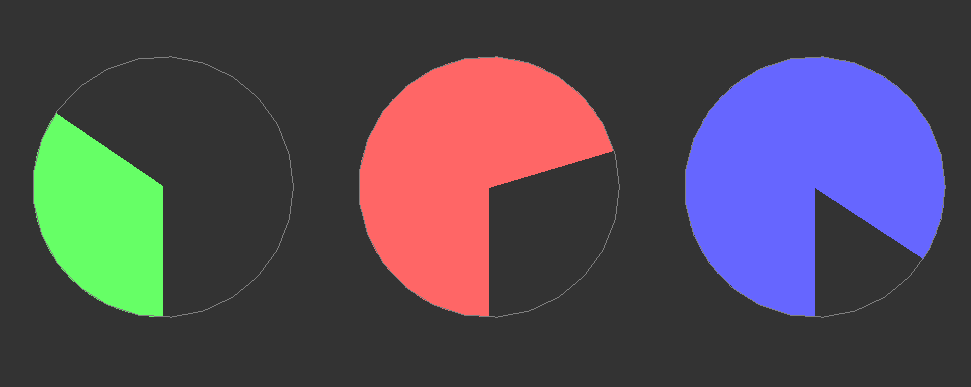
\includegraphics[width=\linewidth]{gfx/06_visual_representation/mpTUI-DialButton.png}
		\caption[Visualisation temporelle à l'aide de chronomètres visuels]{Visualisation temporelle à l'aide de chronomètres visuels de la librairie mp.TUI}
		\label{fig:visual_representation:dialButton}
	\end{minipage}
	\hspace{.02\linewidth}
	\begin{minipage}[t]{0.48\textwidth}
	    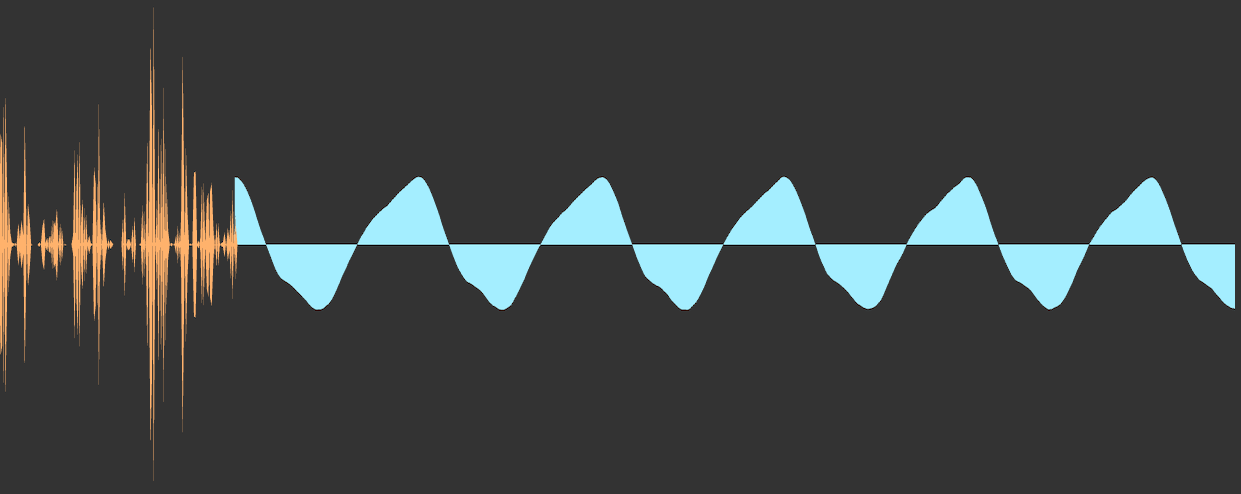
\includegraphics[width=\linewidth]{gfx/06_visual_representation/LAM-DSW.png}
		\caption[Deux échelles temporelles différentes d'un flux audio]{Visualisation du son ``en cours'' et de sa trace accumulée à plus long terme, en utilisant deux échelles temporelles.}
		\label{fig:visual_representation:DSW}
	\end{minipage}
\end{figure}
%------------ Figure : skeuomorphisme et soin du design -----------
\indent Également, l'image peut faciliter la compréhension de processus musicaux sur le long terme, en particulier le déploiement de grandes formes temporelles, qui nécessite une mémoire auditive faisant parfois défaut. Si le son est évanescent, l'image peut en effet laisser une trace sensible, ``s'écrire'' au fur et à mesure de sa performance\footnote{Un tel procédé à été utilisé lors d'un concert de ONE, durant lequel les formes d'ondes des sons joués par chaque musicien étaient vidéo-projetées et s'aggloméraient telle des stalagmites, rendant visible les intensités de jeu de chacun au cours du concert (L'objet LAM.jit.gl.DSW\textasciitilde{} développé à cette fin est disponible dans la LAM-lib).} (cf. figure \ref{fig:visual_representation:DSW}). De manière générale, la ``partition'', qu'elle soit trace du passé ou pré-figuration de ``l'à-venir'', peut se retrouver intégrée dans l'interface instrumentale (cf. chapitre \ref{ch:notation}). Cette ``partition'' n'est pas nécessairement une représentation du temps musical \textit{in extenso}, mais peut être présente sous des formes fragmentées de temps enregistré à la volée ou de séquences pré-programmées.\\
\indent Une autre conséquence du dynamisme de l'interface graphique est la possibilité d'afficher des informations de manière contextuelle, sur le plan spatial (e.g. en affichant des informations uniquement quand on interagit avec une certaine zone de l'interface) comme sur le plan temporel (e.g. en affichant des informations en fonction d'événements en cours).\\
\indent Cette idée de l'interface comme ``cockpit du musicien'' \cite{vertegaal_towards_1996} hérite du contexte technico-scientifique dans lequel les \glspl{DMI} ont vu le jour: les interfaces des premiers ordinateurs ainsi que le matériel de l'ingénierie du son ressemblant bien souvent à celles des cockpits d'avion. Pourtant, si l'image d'un cockpit évoque des gestes de réglage et d'ajustement lents, sur un grand nombre de paramètres mesurés sur des échelles absolues (que cela soit sur un avion ou une table de mixage), la notion d'instrument et de jeu musical appelle de son côté des gestes expressifs, vifs, et souvent sur des échelles relatives\footnote{...comme en témoigne l'importance de valeurs relatives telles que les intervalles ou les nuances (crescendo/decrescendo, ralentendo/accelerando, etc.) dans l'écriture musicale. Cf. également les propos de Serge de Laubier à ce sujet dans l'annexe \ref{appendix:delaubier}.}.

%%%%%%%%%%%%%%%%%%%%%%%%%%%%%%%%%%%%%%%%%
\subsection{L'écran comme interface tangible}

\noindent Dans la chronologie rassemblée par Bill Buxton\footnote{Bien qu'ils ne se soient pas limités à des applications musicales, les développements de Bill Buxton ont été fréquemment appliqués au contrôle de la synthèse et à la lutherie numérique.} \cite{buxton_multi-touch_2007}, il est intéressant de noter que les premières interfaces \textit{multitouch}, développées dans les années 1950, ont été des instruments de musique électroniques\footnote{L'electronic sackbut de Hugh Le Caine, et les claviers de Don Buchla.} (figure \ref{fig:visual_representation:buchla}), utilisant des capteurs capacitifs montés en parallèle, pour le contrôle polyphonique de la synthèse. De même, si le premier \textit{écran multitouch} semble avoir été inventé au Bell Labs en 1984, le premier à avoir été commercialisé pour le grand public a été le Lemur (figure \ref{fig:visual_representation:lemur}) développé par Jazz Mutant en 2003, également destiné au contrôle musical.\\
%------------ Figure : multitouch instruments -----------
\begin{figure}[!htbp]
	\captionsetup{format=plain}%
	\centering
	\begin{minipage}[t]{0.48\textwidth}
		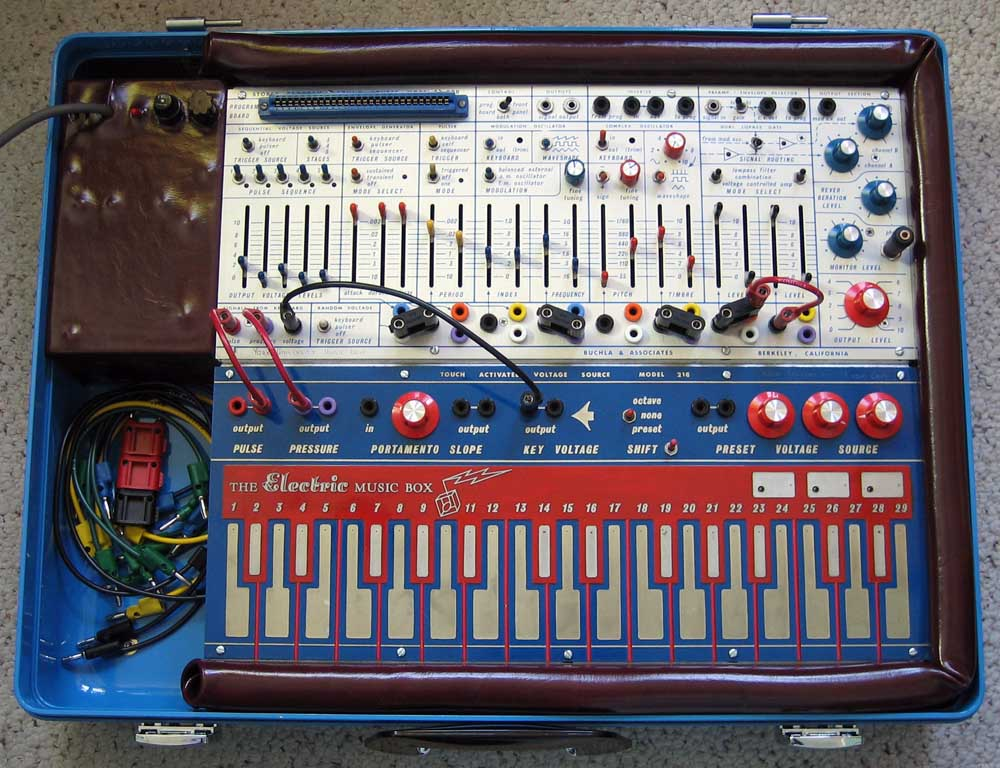
\includegraphics[width=\linewidth]{gfx/06_visual_representation/Buchla_music_easel.jpg}
		\caption[Le clavier multitouch du synthétiseur Buchla music easel]{Le clavier multitouch du synthétiseur Buchla music easel (1972).}
		\label{fig:visual_representation:buchla}
	\end{minipage}
	\hspace{.02\linewidth}
	\begin{minipage}[t]{0.48\textwidth}
	    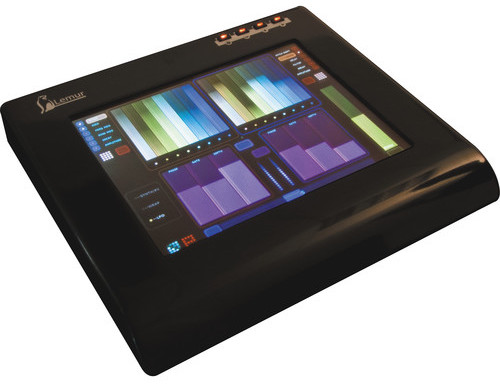
\includegraphics[width=\linewidth]{gfx/06_visual_representation/Lemur.jpg}
		\caption[Le Lemur de Jazz Mutant et son écran multitouch]{Le Lemur de Jazz Mutant et son écran multitouch (2003).}
		\label{fig:visual_representation:lemur}
	\end{minipage}
\end{figure}
%------------ Figure : multitouch instruments -----------
\indent Les interfaces tangibles se sont multipliées dans les appareils grands public au tournant du siècle, notamment sous l'impulsion de projets de recherche tels que ceux du \textit{Tangible médias Group} dirigé par Hiroshi Ishii au médias Lab du \gls{MIT}. Si un certain nombre de gestes (la notion de geste étant ici souvent réduite au gestes des doigts, voire du pouce, de l'index et du majeur seulement) sont devenus des standards pour l'interaction sur ce type d'interfaces (tel le \textit{pinch-zoom}, le \textit{swipe}, etc.), la recherche sur les interactions possibles reste un domaine récent et encore largement inexploré. Les écrans multitouch offrent de nombreux avantages qui ont déjà été soulignés par Bill Buxton \cite{buxton_multi-touch_2007} et Sergi Jorda \cite{jorda_digital_2005}, notamment :
%-------------
\vspace{-1em}
\begin{itemize}[noitemsep]
	\item l'utilisation possible de plusieurs doigts, plusieurs mains, plusieurs personnes en même temps, en comparaison de la souris, qui permet une interaction polyphonique, parallèle plutôt que séquentielle;
	\item la cohésion entre le contrôle d'un objet et sa représentation et la relation sensuelle d'intimité qui se créé en l'absence de distance entre l'objet virtuel et celui/celle qui le manipule.
\end{itemize}
%-------------
\noindent La cohésion entre la représentation et le contrôle d'un objet virtuel\footnote{... qui, rappelons-le, n'est qu'une ``synchrèse'', c'est-à-dire un artéfact liant les deux phénomènes par leur concommittence spatio-temporelle.} facilite l'intuitivité de l'interface en abolissant la distance entre ces deux aspects de l'interaction. Au-delà de cet intérêt ergonomique, cela permet d'imaginer de nouveaux scénarios d'interactions dynamiques. Même de simples interactions usuelles, comme celle de la bureautique (sliders, boutons, etc), peuvent être ré-inventées avec des comportements alternatifs, dans une perspective d'utilisation musicale, comme nous le verrons plus loin.\\
\indent Cette idée est notamment poursuivie dans le domaine des \gls{IHM}, avec le dessein d'intégration du numérique dans les objets du monde physique, telle que présenté notamment dans l'article ``Tangible Bits'' d'Ishii et Ullmer \cite{ishii_tangible_1997} et reprise par Sergi Jordà dans les 25 principes qu'il adopte pour le développement de la ReacTable\footnote{``For including realtime interactive visualizations and, at the same time, overcoming
mouse limitations without adding indirections, interfaces should be able to reflect their own states and behaviors. They should integrate, like the abacus, both representation and control.'' \cite{jorda_digital_2005}}.\\
\indent Ce faisant, la cohésion entre le geste et la représentation ``acquise'' dans les écrans tactile laisse la place à des scénarios d'interaction subersifs (sur le geste subversif, cf. section \ref{sec:gesture:subversion}) qui se jouent de cette synchrèse artificielle\footnote{Voir par exemple la série de performances ``Screen to screen'' de l'artiste Vincent Brocquaire, basées sur cette duplicité de l'écran/interface. \url{http://www.vincentbroquaire.com/screen-to-screen.html}}.\\


%%%%%%%%%%%%%%%%%%%%%%%%%%%%%%%%%%%%%%%%%
\subsection{Topologie dynamique}

\subsubsection{Repères statiques, amovibles, dynamiques}

%------------------- Visual markers -----------------------
\begin{figure}[!htbp]
	\captionsetup{format=plain}%
	\makebox[\linewidth][c]{%
		\begin{subfigure}[b]{.34\textwidth}
			\centering
			\includegraphics[width=.95\textwidth]{gfx/06_visual_representation/guitar-frette.jpg}
			\caption{\textbf{statiques} repères sur un manche de guitare}
		\end{subfigure}%
		\begin{subfigure}[b]{.34\textwidth}
			\centering
			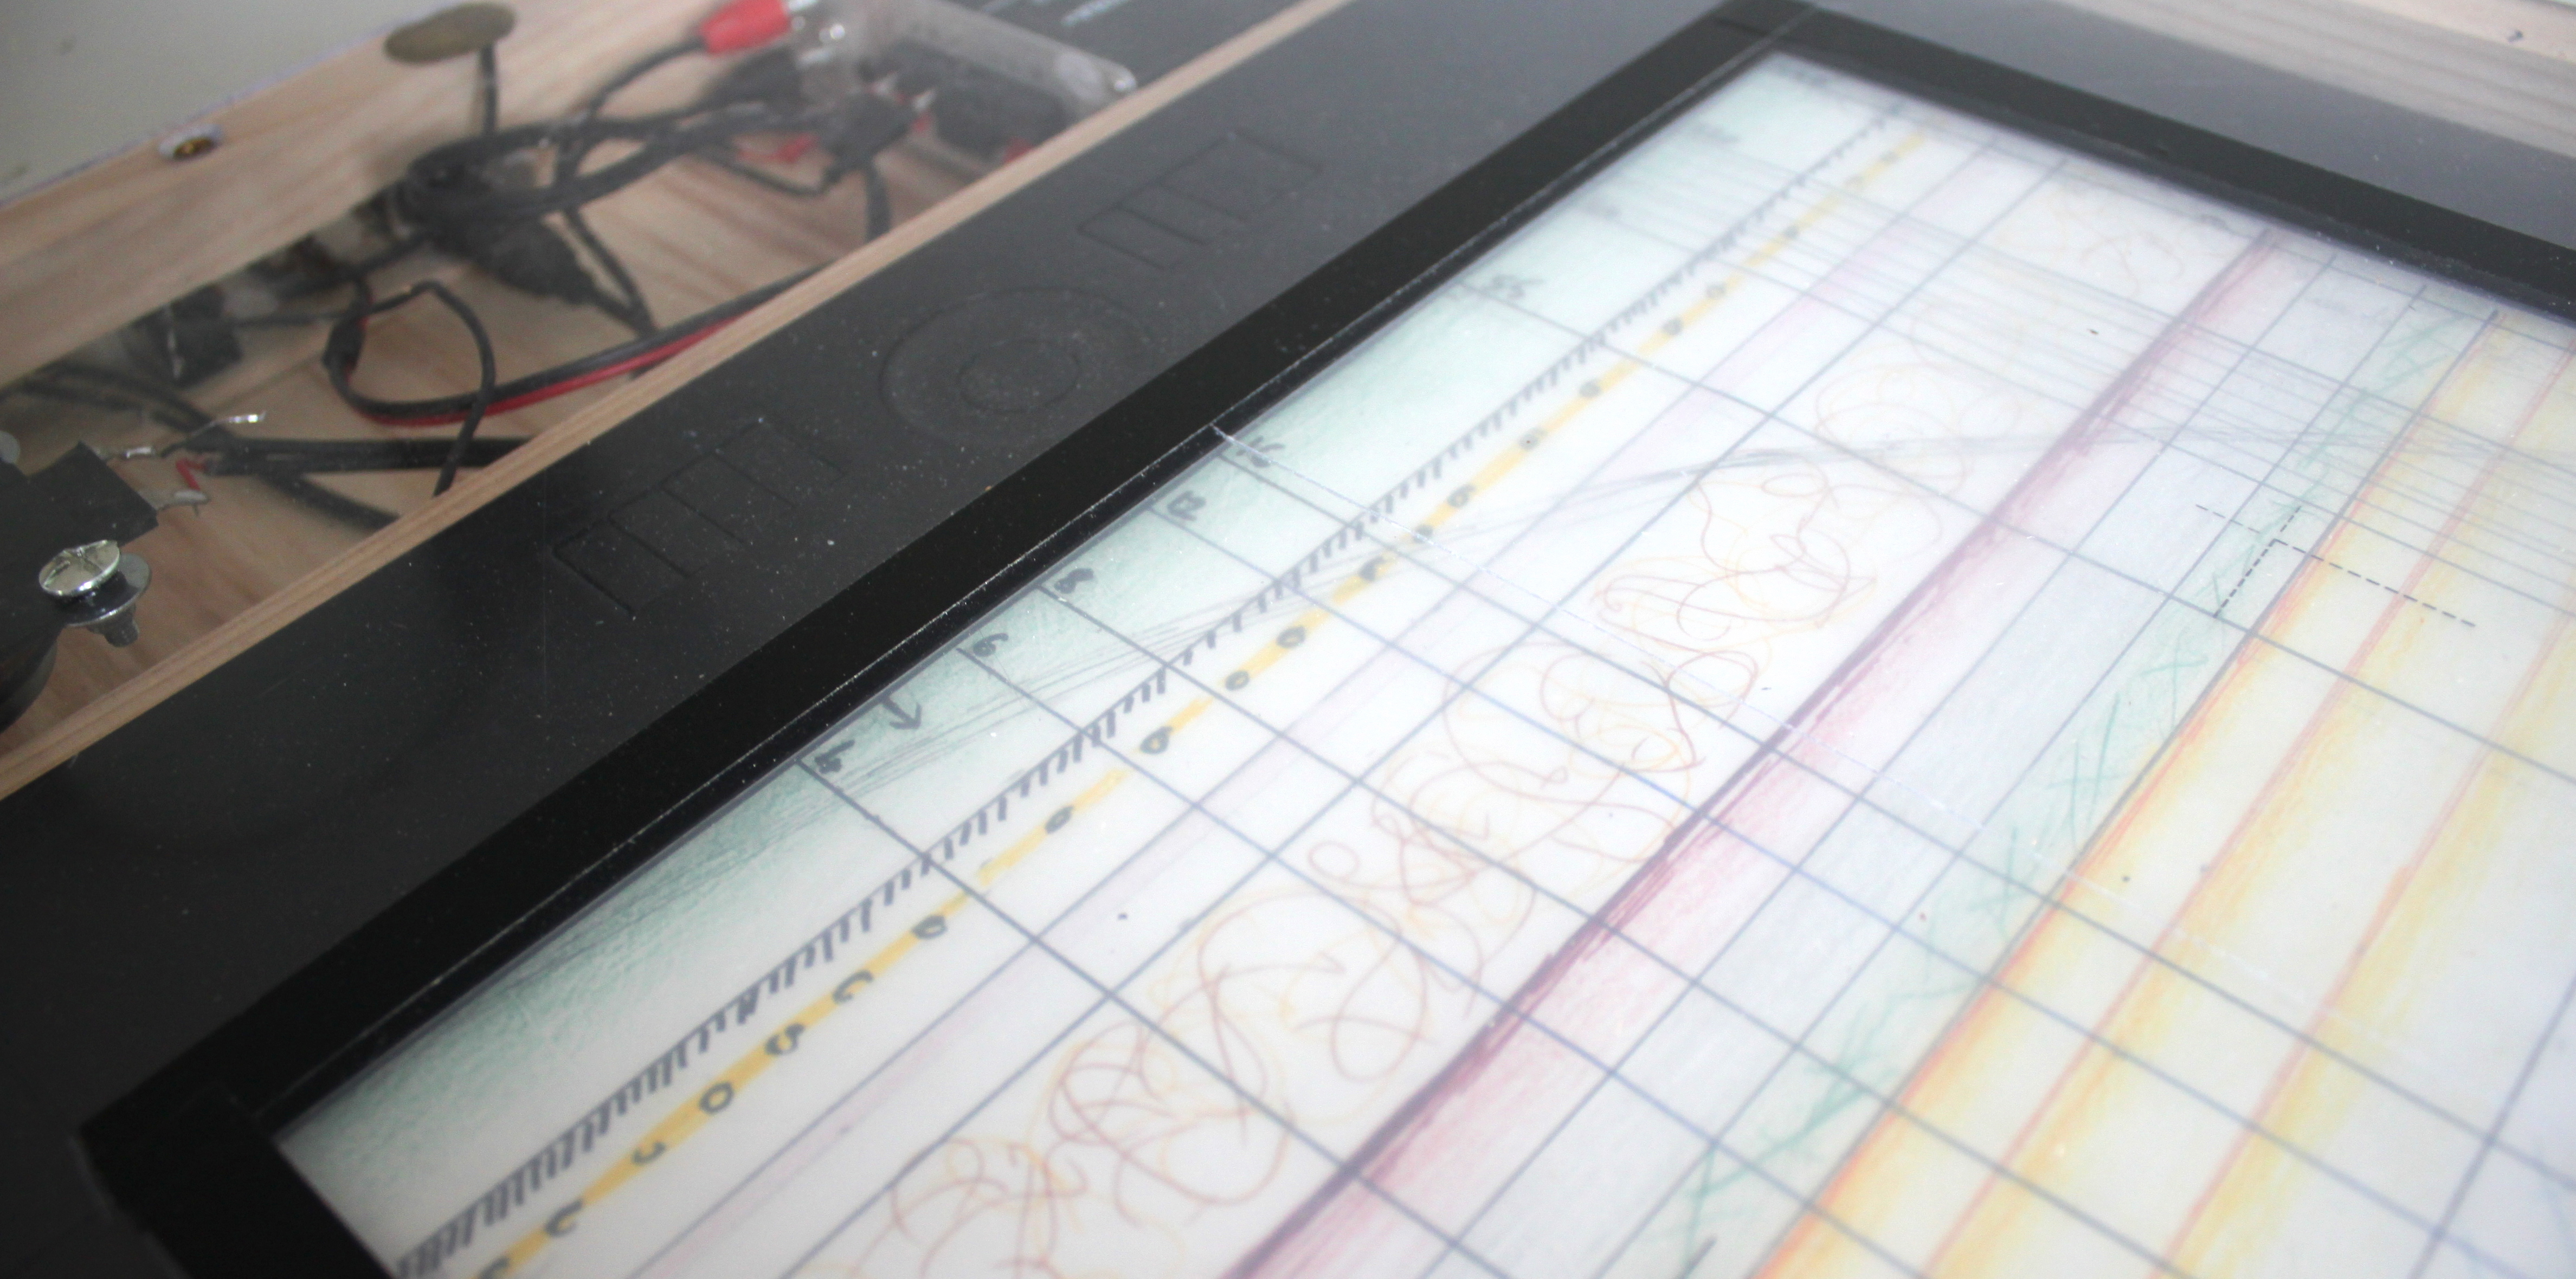
\includegraphics[width=.95\textwidth]{gfx/06_visual_representation/filigramophone-visualMarkers.jpg}
			\caption{\textbf{amovibles}, calque sur une tablette graphique}
		\end{subfigure}%
		\begin{subfigure}[b]{.34\textwidth}
			\centering
			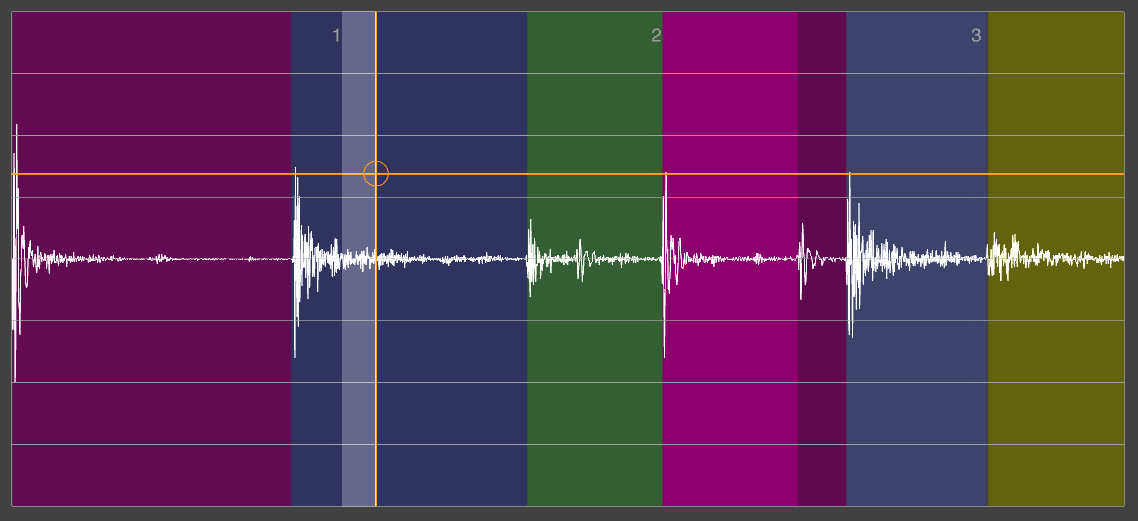
\includegraphics[width=.95\textwidth]{gfx/06_visual_representation/mpTUI-visualMarkers.png}
			\caption{\textbf{dynamiques}, segmentation d'un échantillon sur un écran multitouch}
		\end{subfigure}%
	}
	\caption{Repères visuels sur différentes interfaces instrumentales.}
	\label{fig:visual_representation:visual-markers}
\end{figure}
%------------------- Visual markers -----------------------

\noindent Le positionnement des différents capteurs de l'interface d'un \gls{DMI} définit une topologie de l'interaction qui peut être soulignée par des repères visuels (cf. figure \ref{fig:visual_representation:visual-markers}). On peut ainsi distinguer trois cas de figure, concernant le positionnement de ces repères visuels :
\vspace{-1em}
\begin{itemize}[noitemsep]
	\item \textbf{statique} : les repères sont fixes et l'algorithme sous-jacent pourra être ``ré-accordé'' dans les limites imposées par cette configuration (e.g. il est possible de changer la tension des cordes d'une guitare, sans que la position des frettes soient invalidée);
	\item \textbf{amovible} : les repères peuvent être changés ``physiquement'', soit que leurs positions soient réglables (e.g. comme c'est le cas pour les frettes du sitar), soit qu'ils soient interchangeables (e.g. les différentes revêtements de l'interface \textit{Joué} ou du \textit{Sensel Morph}, ou le calque glissable dans une tablette graphique);
	\item \textbf{dynamique} : cette solution est rendue possible sur les écrans tactiles, mais n'offre pour l'instant pas les qualités haptiques de repères en relief permises par les repères statiques ou amovibles\footnote{Un certain nombre de prototypes d'écrans à formes dynamiques ont été développés cette dernière décennie (voir \cite{follmer_inform_2013, siu_shapeshift_2018}), mais restent encore très rustiques et ne semblent pas encore prêts pour une diffusion commerciale.}.
\end{itemize}


\subsubsection{Nouvelles formes et nouvelles fonctions}

\noindent De nombreuses règles ont été formulées dans le domaine du design, de l'architecture, des \gls{IHM}, et de la visualisation de données, telles que le célèbre adage ``la forme suit la fonction'', pris comme paradigme dans le design et l'architecture moderne, autant que dans le design des interfaces graphiques. Ces règles de design prônent généralement le minimalisme, la lisibilité et l'efficacité du design. L'ouvrage d'Edward W. Tufte ``The visual display of quantitative information'' \cite{tufte_visual_2001}, une des principales références dans le domaine de la visualisation de données, rappelle ainsi ces ``Principes de l'Excellence Graphique'' :
\vspace{-1em}
\begin{itemize}[noitemsep]
	\item l'excellence graphique est une présentation bien conçue de données intéressantes — une affaire de \textit{substance}, de \textit{statistiques} et de \textit{design};
	\item l'excellence graphique consiste en la communication claire, précise et efficace d'idées complexes;
	\item l'excellence graphique est ce qui donne le plus grand nombre d'idées dans le temps le plus court, avec le moins d'encre possible et dans le plus petit espace;
	\item l'excellence graphique est presque toujours multivariée;
	\item elle requiert de dire la vérité sur les données.
\end{itemize}

\noindent On retrouve des règles similaires dans les (nombreuses) préconisations concernant le design d'interfaces graphiques, guidées par une recherche de fonctionnalité, lisibilité et transparence maximales. Bien que toutes ces règles puissent être utiles pour le design de la partie graphique d'un \gls{DMI}, il faut cependant garder en tête que les instruments de musique ne sont pas des interfaces dont la raison d'être est définie par leur fonctionnalité (on n'achète pas un instrument pour se rendre la vie plus facile), et que les notions d'\textit{efficacité}, de \textit{lisibilité} et de \textit{vérité} y sont particulièrement sujettes à caution.


\subsubsection{Mettre les doigts dans la prise}
% \begin{wrapfigure}{R}{0.5\textwidth}
% 	\captionsetup{format=plain}%
% 	\centering 
% 	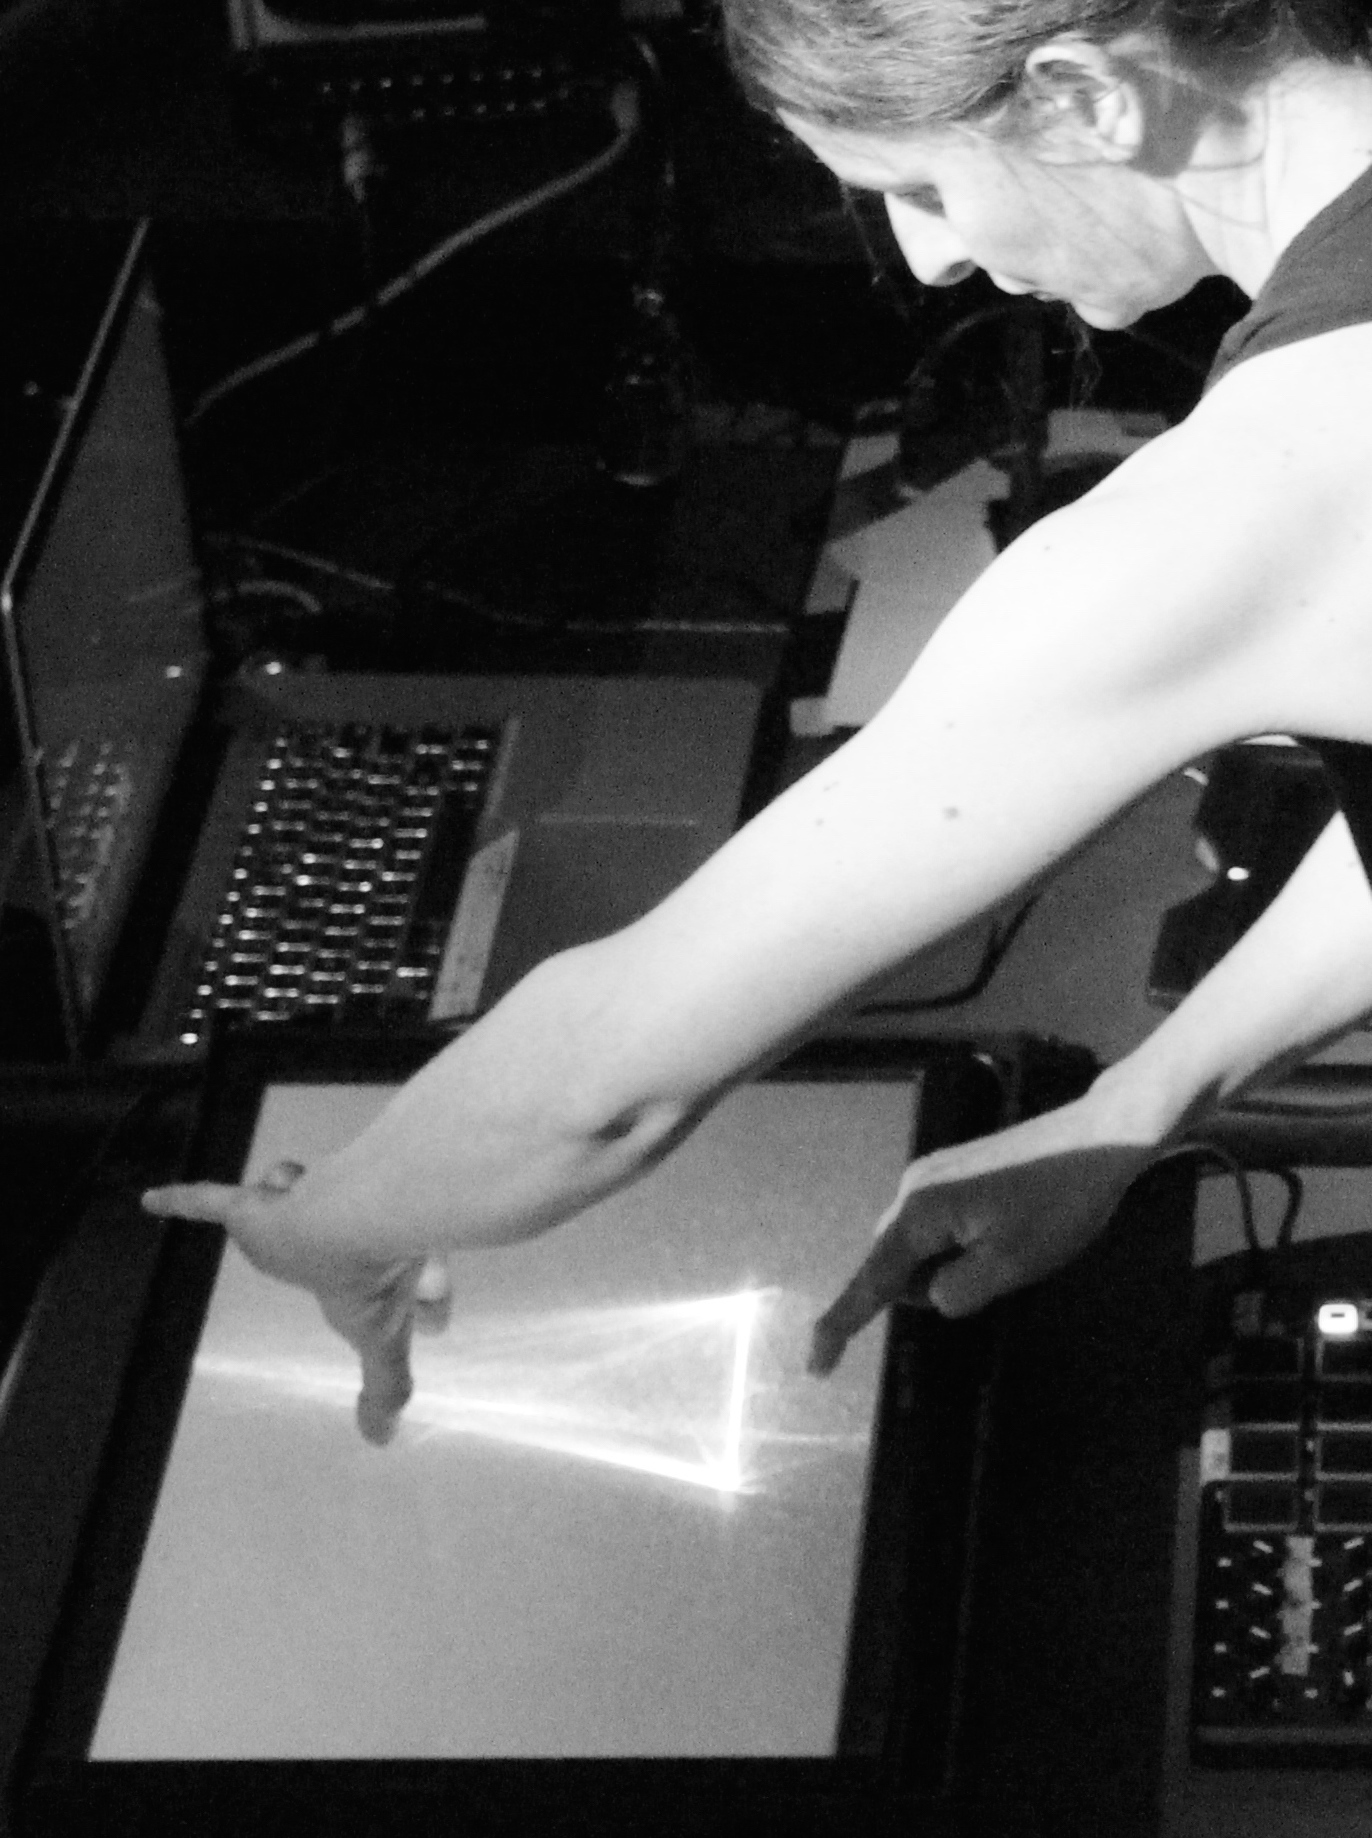
\includegraphics[width=0.48\textwidth]{gfx/06_visual_representation/Xypre-Live.jpg}
% 	\caption[Modèle intermédiaire stochastique manipulé sur écran]{Modèle intermédiaire stochastique manipulé directement sur écran, durant la performance FIB\_R.}
% 	\label{fig:visual_representation:xypre-live}
% \end{wrapfigure}
% \par
%-------------------------- Figure : Fingers on MID ------------------------
\begin{figure}[!htbp]
	\captionsetup{format=plain}%
	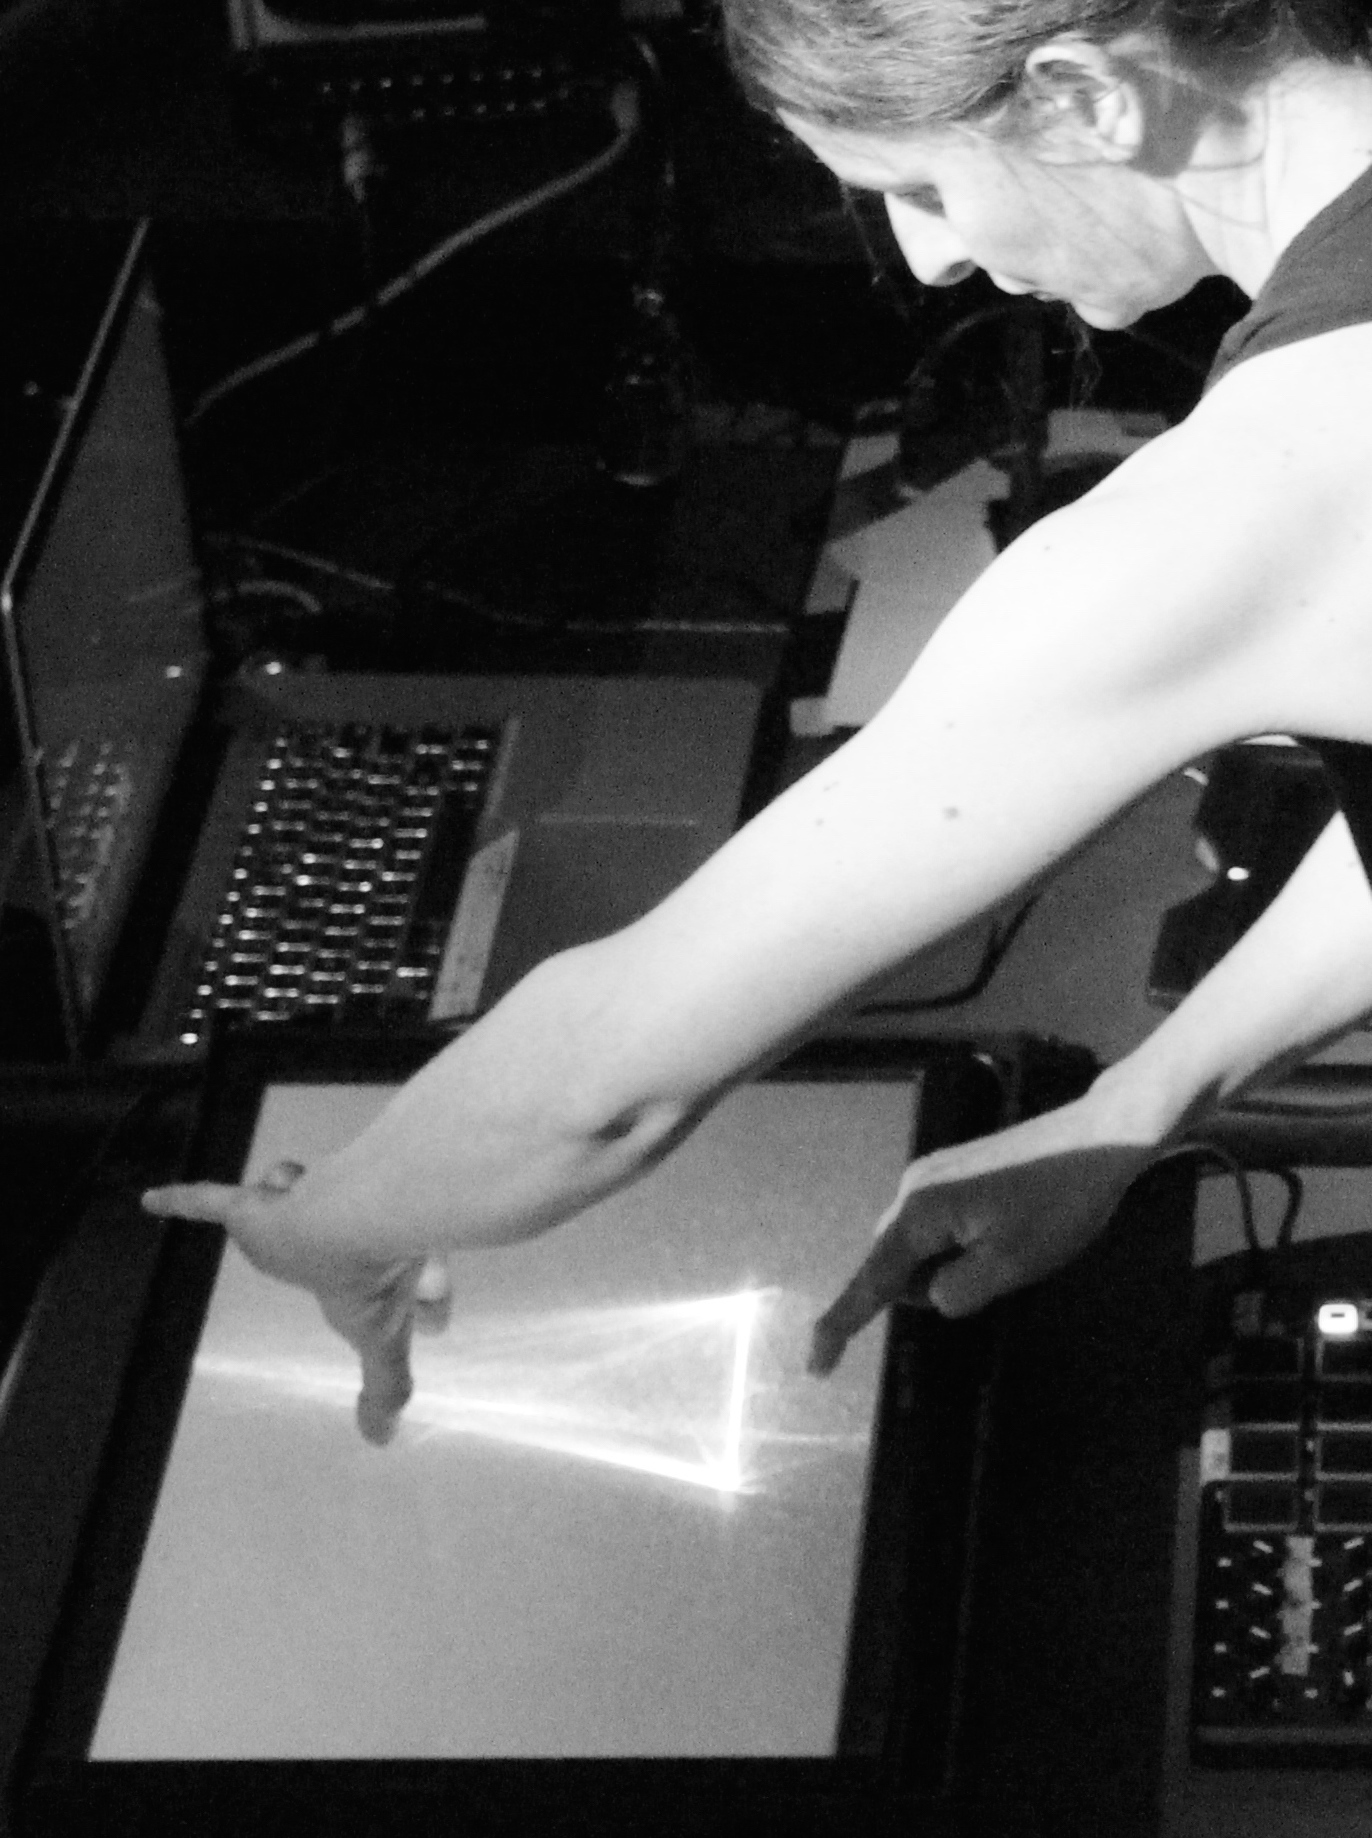
\includegraphics[width=\textwidth]{gfx/06_visual_representation/Xypre-Live.jpg}
	\caption[Modèle intermédiaire stochastique manipulé sur écran]{Modèle intermédiaire stochastique manipulé directement sur écran (interface Xypre présentée au chapitre \ref{ch:interfaces}), durant la performance \textit{FIB\_R}.}
	\label{fig:visual_representation:xypre-live}
\end{figure}
%-------------------------- Figure : Fingers on MID ------------------------

\noindent Si dans un instrument acoustique, l'énergie se transmet des gestes du musicien à l'instrument qui produit le son, cette chaîne d'interaction peut se retrouver perceptivement renversée dans les \glspl{DMI}. Le processus, ou ``modèle intermédiaire'' (cf. \ref{sec:algorithms:MID}) qui \textit{tourne} sur la machine possède son propre mouvement autonome, que les doigts viennent perturber, infléchir, canaliser, étouffer, aiguiser, filtrer... La représentation visuelle de modèles intermédiaires dynamiques vient rendre manifeste ces \textit{forces invisibles}\footnote{\iquote{En art, et en peinture comme en musique, il ne s’agit pas de reproduire ou d’inventer des formes, mais de capter des forces. (...) La tâche de la peinture est définie comme la tentative de rendre visibles des forces qui ne le sont pas. De même la musique s’efforce de rendre sonores des forces qui ne le sont pas.} Gilles Deleuze \cite{deleuze_francis_1981} p 57.} et appelle ainsi des gestes \textit{en réponse} aux mouvements internes du modèle, qui redéfinit en permanence l'espace de son interaction, dont la topologie n'est pas donnée d'avance et qu'il s'agit apprivoiser (cf. figure \ref{fig:visual_representation:xypre-live}).


%\subsection*{Extra material : todo remove}

% Apprendre indépendamment de la transposition
% \iquote{I love the piano sound but not the difficulty of learning the variations from one key to another.  The LinnStrument with its 4th tuning avoids all of those issues.} Jeff Moen about the linnstrument (\url{http://jeffmoen.com/how_i_got_here.html})

%%%%%%%%%%%%%%%%%%%%%%%%%%%%%%%%%%%%%%%%%
\section{La librairie mp.TUI pour Max}

%\todo{Rajouter des figures pour édition directe (shipped with handles) et modèle voronoi}

\noindent La bibliothèque mp.TUI\footnote{Sources disponible sur \url{https://github.com/LAM-IJLRA/ModularPolyphony-TUI}.} pour Max propose des composants graphiques permettant le contrôle et la représentation d'une interaction polyphonique et modulaire. Elle offre également (et surtout) un environnement ouvert pour la programmation de nouveaux objets graphiques et de nouvelles interactions en mettant à disposition des briques de base prenant en charge les fonctions élémentaires usuelles. Cette section présente une brève revue des outils existants et des motivations avant de détailler le fonctionnement de la librairie.

\subsection{Motivations}

\subsubsection{Antécédants} 

\noindent Plusieurs développements ont été réalisés depuis 2003 permettant de contrôler, de différentes manières, des patchs Max via une interface \textit{multitouch}. Parmi les réalisations, on peut noter notamment :
\vspace{-1em}
\begin{itemize}[noitemsep]
	\item \textbf{le Lemur} : une interface \textit{multitouch} personnalisable développé par la société JazzMutant entre 2003 et 2011, d'abord sur une interface hardware dédiée avant d'être portée sous la forme d'une application pour tablettes et smartphones\footnote{distribuée par la société Liine \url{https://liine.net/en/products/lemur}}. Cette interface était pionnière, à la fois à une époque où le \textit{multitouch} grand public était naissant, et par la possibilité de personnaliser l'interface à l'aide d'un éditeur tournant sur un ordinateur standard. La personnalisation était cependant limitée au fait de choisir les composants graphiques parmi un ensemble de composants alignables sur une grille;

	\item \textbf{la librairie MMF} : ``Max Multitouch Framework''\footnote{Vidéo présentant MMF: \url{https://www.youtube.com/watch?v=EEkj85GU_is}} développé par Mathieu Chamagne\index[people]{chamagne@Chamagne, Mathieu} dans le cadre du projet \gls{ANR} Virage (2008-2010), qui permettait de contrôler certains éléments de \gls{GUI} de Max. La contrainte principale réside dans le fait que le contrôle des éléments de \gls{GUI} de Max est assez gourmand en \gls{CPU} et rend difficile l'usage de plusieurs doigts;

	\item \textbf{TouchOSC} : développé en 2008, touchOSC\footnote{\url{https://hexler.net/products/touchosc}} est basé sur les principes du Lemur mais développé comme une application pour tablette et smartPhones, permettant de renvoyer des données \gls{MIDI} ou \gls{OSC};

	\item \textbf{Mira} : En 2013, Sam Tarakajian présente Mira\footnote{dont la vidéo de présentaion est intéressante à plus d'un titre \url{https://vimeo.com/63846055}}, qui sera distribué ensuite par Cycling'74\footnote{\url{https://cycling74.com/products/mira}}, la société développant Max. Mira simplifie grandement la connexion entre un iPad et un patch Max dans la mesure où les éléments de \gls{GUI} d'un patch Max sont directement transposés sur l'interface \textit{multitouch}, sans qu'il y ait besoin de recréer des connexions manuellement entre deux interfaces différentes, comme cela pouvait être le cas avec le Lemur ou TouchOSC;

	\item \textbf{Max multitouch} Enfin, Cycling'74 a considérablement amélioré la mécanique de patching depuis la version 8, et a commencé fin 2018 l'implémentation native du \textit{multitouch} dans l'éditeur de patch, pour l'instant limitée à un certain nombre d'objets et à la version Microsoft Windows.
\end{itemize}

\subsubsection{De la nécessité de réinventer la roue} 

\noindent À la vue de ces développements, on peut légitimement se demander quel est l'intérêt de développer une librairie graphique pour le \textit{multitouch} dans Max. La réponse est essentiellement liée à la conviction que les interfaces graphiques, tout comme le domaine du mapping, ne consistent pas en un simple agencement de composants standards, mais en un champ ouvert à la créativité, pour développer de nouvelles représentations interactives. \\
\indent Si l'on prend l'exemple d'un objet aussi basique et courant qu'un \textit{slider}; l'objet paraît \textit{a priori} simple et univoque. Pourtant, si l'on détaille le mécanisme de corrélation entre le geste et le comportement de l'objet, on s'aperçoit rapidement que de nombreux scénarios sont non-seulement possibles, mais pertinents selon le contexte\footnote{Un exemple notoire sur l'usage du \textit{slider} est l'introduction, en 2011, de ce qu'Apple nomma ``scrolling naturel'', en inversant le sens de défilement des documents pour répondre aux nouvelles interfaces tactiles et en balayant plus de 25 ans de convention d'usage. Les réactions fûrent largement hostiles au début, mais le nouvel usage finit par être non-seulement accepté mais également considéré comme plus naturel. Dans ce cas précis, la question se pose sur la partie du slider sur laquelle on agit : le contenu ou bien le cadre. Si l'on prend un équivalent dans le domaine de l'audio, le déplacement d'une tête de lecture dans un échantillon, tel que couramment représenté dans les interfaces de synthèse granulaire, est aussi approprié que l'idée de déplacer l'échantillon ``sous'' la tête de lecture, et qui constitue la manière dont fonctionnait les lecteurs à bande.}, de sorte que les implémentations d'interactions basiques --~telle que celle d'un slider~-- dans la plupart des logiciels de bureautique ne sont pas nécessairement les plus adaptées au contrôle musical. Ainsi, un musicien utilisera une telle interface linéaire avec \underline{tous ses doigts}, par exemple pour jouer des intervalles mélodiques, usage pour lequel la mémoire des intervalles s'avère très ergonomique. Il suffit de tester le fonctionnement des sliders sur les tablettes dans la plupart des applications pour constater que ce genre d'interaction n'y est, sans surprise, pas prévu. De même, la plupart des logiciels contraignent l'orientation des composants graphiques selon les axes vertical et horizontal (c'est pour l'instant le cas de toutes les librairies sus-mentionnées), en se basant sur l'usage habituel de l'écran bureautique, qui se lit de haut en bas et de gauche à droite\footnote{On peut noter le choix original d'un design basé sur le cercle dans la ReacTable, inspiré de celui de l'AudioPad développé en 2002 au \gls{MIT}, pour faciliter un usage collectif.}.\\
\indent Ainsi, la prise en charge native du \textit{multitouch} dans l'interface de Max ne saurait être satisfaisante en terme créatif si elle ne laisse pas les relations entre les objets graphiques et le geste ouvertes à la reprogrammation. 

\subsection{Utilisation de MP pour le contrôle \textit{multitouch} de GUI}

\noindent Comme son nom l'indique, la librairie mp.TUI est construite sur le protocole MP (cf. section \ref{sec:algorithms:MP}). Elle fournit un cadre, basé sur les logiques de patching de Max, pour créer de nouveaux composants \gls{GUI} \textit{multitouch} dans un contexte graphique OpenGL et surmonter certaines limitations de l'interface graphique native de l'environnement de patching de Max. Par exemple, les interfaces graphiques sont généralement orientées sur une disposition horizontale/verticale avec une orientation de lecture du haut vers le bas alors qu'on peut souhaiter avoir plusieurs orientations, comme dans la situation présentée sur la figure \ref{fig:visual_representation:multi_orientation}. La superposition de divers composants peut nécessiter des couleurs et des transparents personnalisés, et l'on peut souhaiter inclure des interfaces visuelles plus complexes que les curseurs et les boutons, par exemple des particules, des vidéos, des modèles 3d, des shaders (cf. figure \ref{fig:visual_representation:phonetogramme}), etc. Les composants de la bibliothèque sont un ensemble d'abstractions de trois types :
\vspace{-1em}
\begin{itemize}[noitemsep]
	\item \textbf{des composants système}, qui implémentent les fonctions de base permettant la communication entre les objets de la \gls{GUI}. En particulier, l'objet \verb|mp.TUI.hub| récupère les données de la souris ainsi que les messages \gls{TUIO} reçus par \gls{UDP} et les envoie aux composants graphiques sélectionnés;
	\item \textbf{des éléments de GUI}, qui sont des instances prêtes à l'emploi de composants courants ou moins courants tels que curseurs, claviers, graphes, etc.;
	\item \textbf{des outils}, un ensemble d'abstractions qui permettent de créer facilement de nouveaux composants en proposant des fonctions utiles pour la conception d'interaction (transformation de la visualisation, gestion de la polyphonie sur un élément, interaction tels que pinch-zoom, calcul de dérivées, etc.).
\end{itemize}

\subsection{Les composants de la librairie mp.TUI}

\noindent Les composants utilisent des transformations géométriques hiérarchiques\footnote{à l'aide de l'objet jit.anim.node de Max}, qui permettent d'obtenir des coordonnées relatives à l'écran ou au composant, indépendamment de la position, de l'échelle et de l'orientation du composant. Cela permet également de créer des groupes de composants, comme on le ferait dans n'importe quel logiciel d'édition graphique vectoriel. Suivant la nature empirique de la lutherie numérique revendiquée ci-dessus, un ``mode édition'' est également disponible pour manipuler rapidement à la main la position, l'échelle et l'orientation des composants de l'interface utilisateur (figure \ref{fig:visual_representation:groups_patch} et \ref{fig:visual_representation:groups}).

%-------------------------- Figure : phonétogramme ----------------------------------
\begin{figure}[!htbp]
	\captionsetup{format=plain}%
	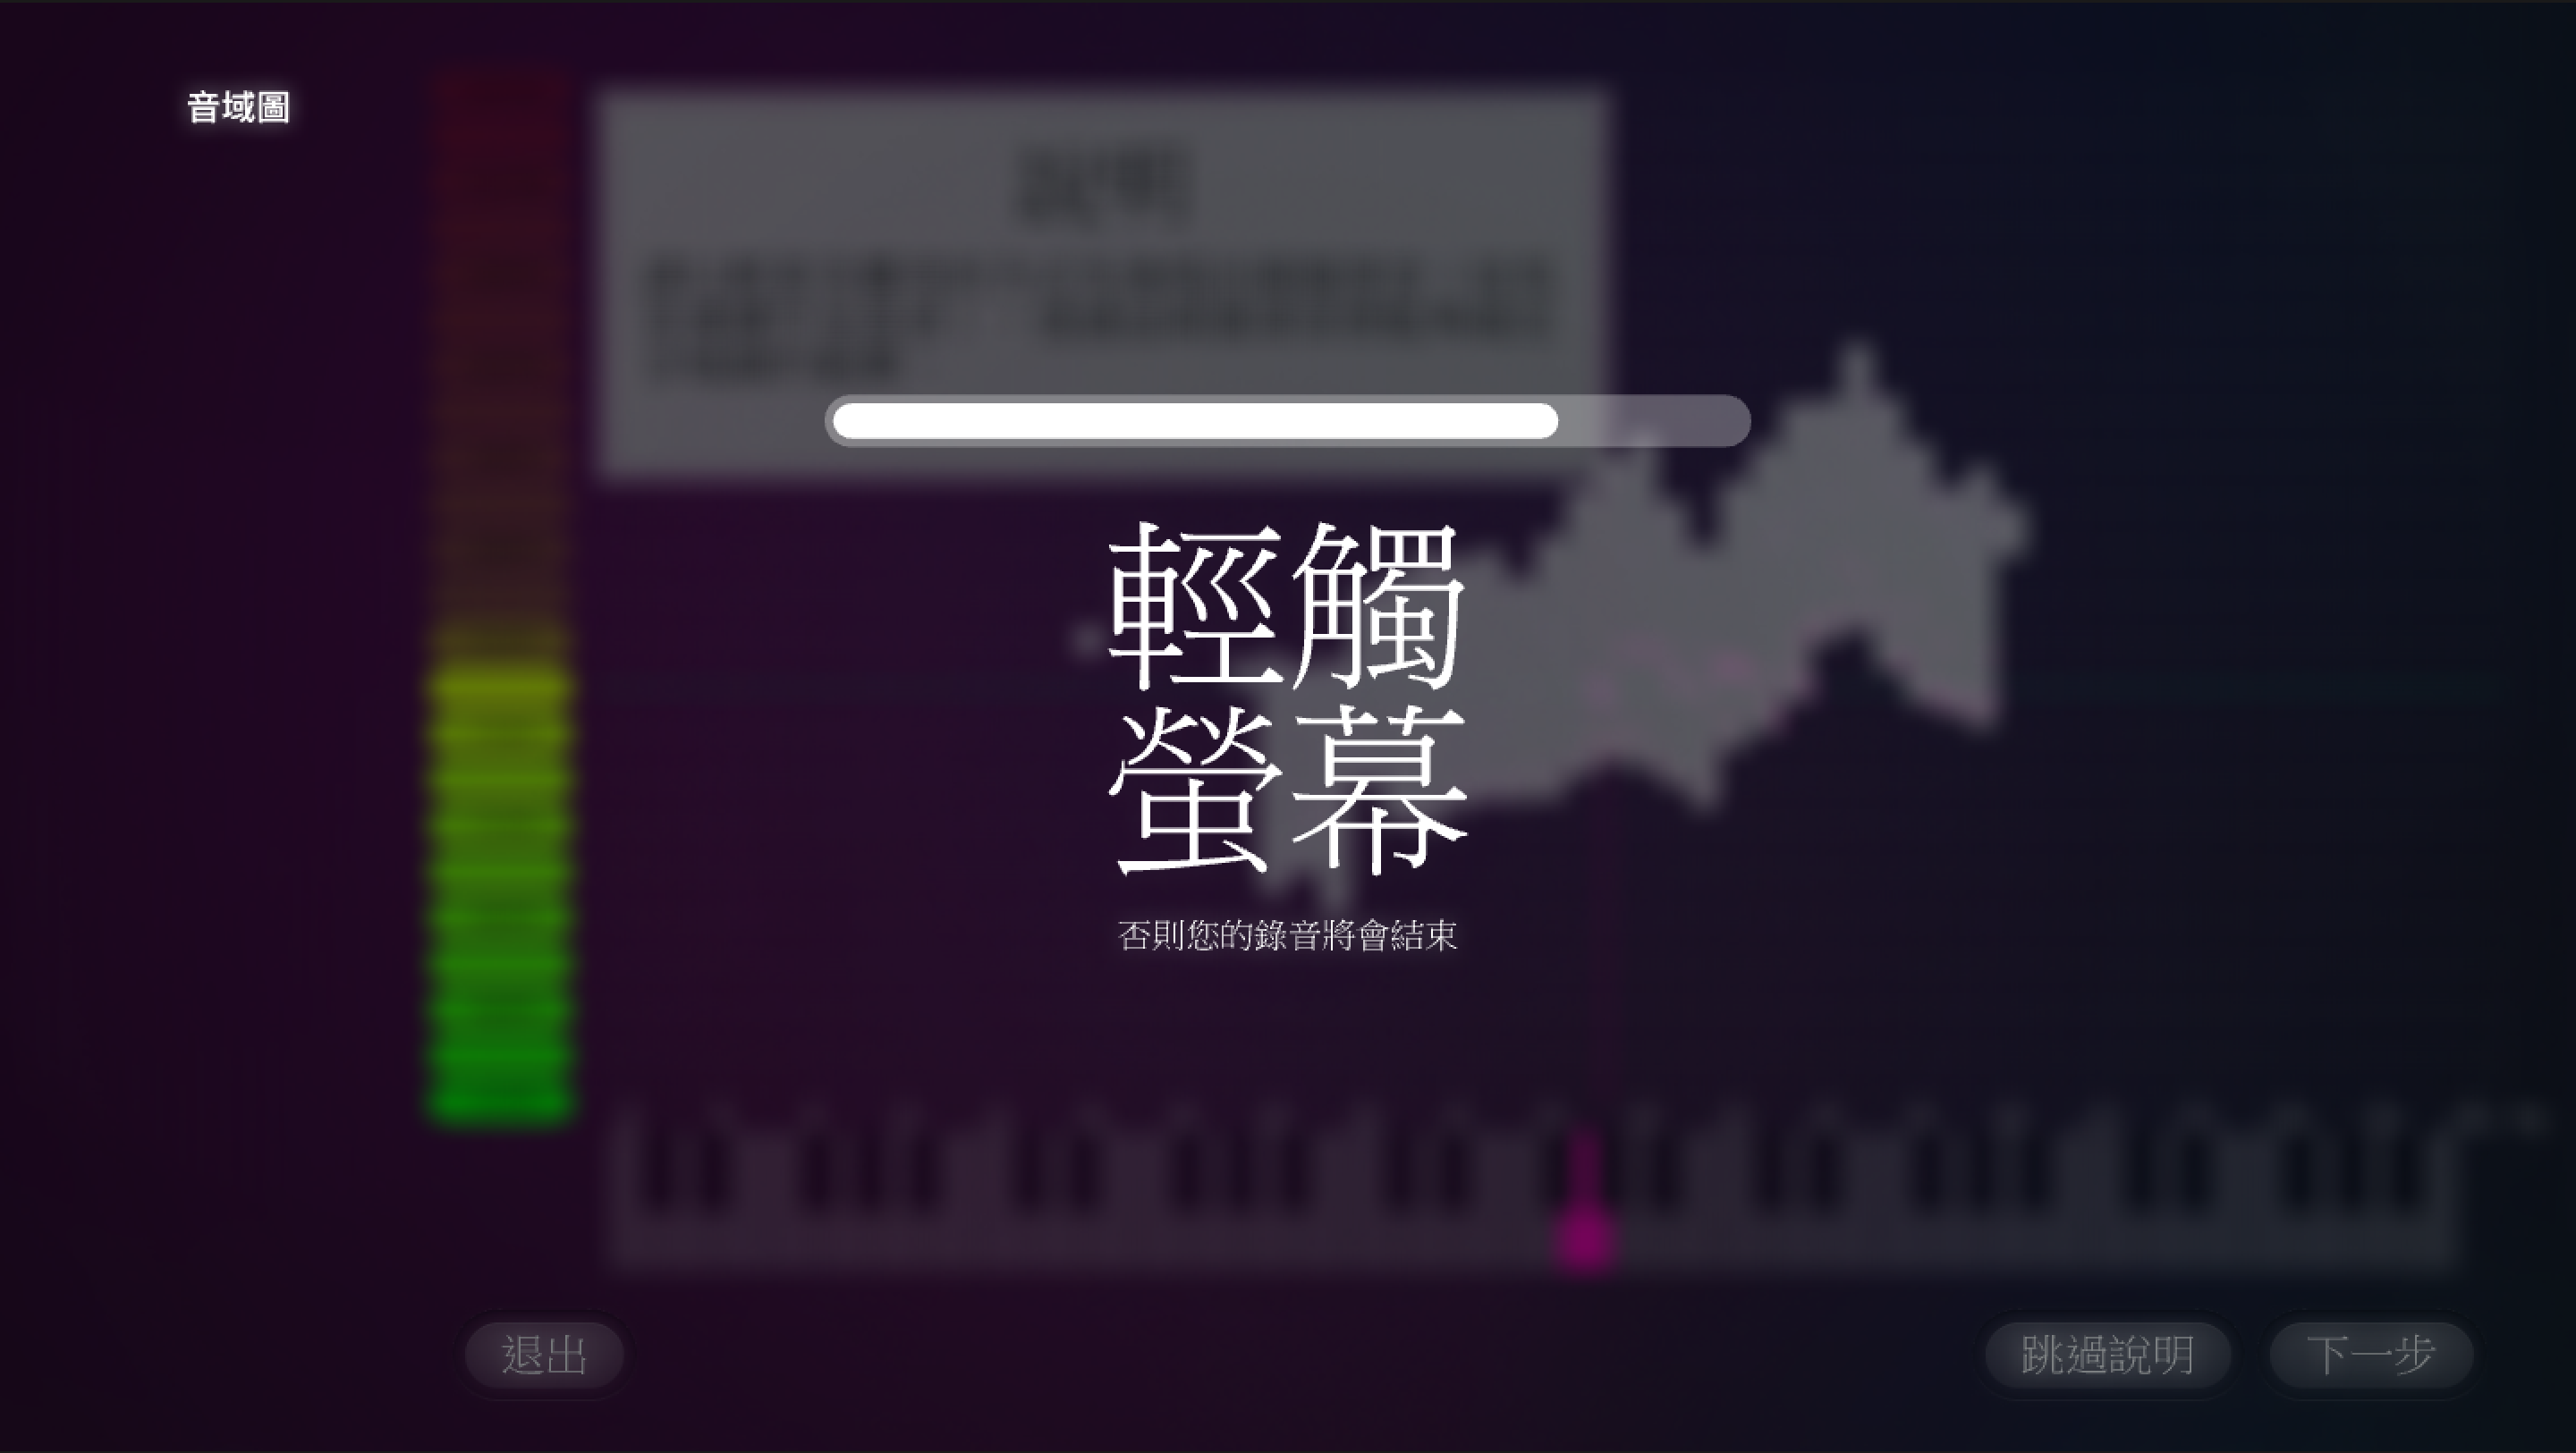
\includegraphics[width=\textwidth]{gfx/06_visual_representation/Phonetogramme.png}
	\caption[``Le phonétogramme'', une application réalisée à l'aide de la librairie mp.TUI]{``Le phonétogramme'', une application muséographique conçue pour la Cité des Sciences, dont la GUI est réalisée avec la librairie mp.TUI.}
	\label{fig:visual_representation:phonetogramme}
\end{figure}

\noindent La possibilité de concevoir des objets audiovisuels en Max en étroite relation avec la programmation de l'interaction entre le geste, l'audio et le visuel permet de les intégrer dans des scénarios dynamiques personnalisés : histoires narratives pour des ateliers éducatifs avec des enfants, scénarios réactifs, visualisations personnalisées pour les malvoyants, expositions muséographiques avec chartes graphiques spécifiques, adaptation réactive aux formats d'écrans, graphismes expérimentaux pour l'esthétique des performances artistiques live, etc.
%------------------ Figure : mp.TUI : simple slider ---------------------
\begin{figure}[!htbp]
	\makebox[\linewidth][c]{%
		\begin{subfigure}[b]{.5\textwidth}
			\centering
			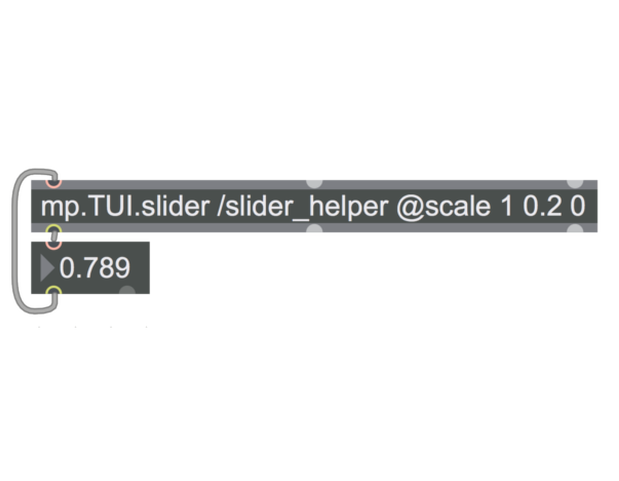
\includegraphics[width=.95\textwidth]{gfx/06_visual_representation/mpTUI_slider-patcher.png}
			\caption{L'objet Max créant un slider}
		\end{subfigure}%
		\begin{subfigure}[b]{.5\textwidth}
			\centering
			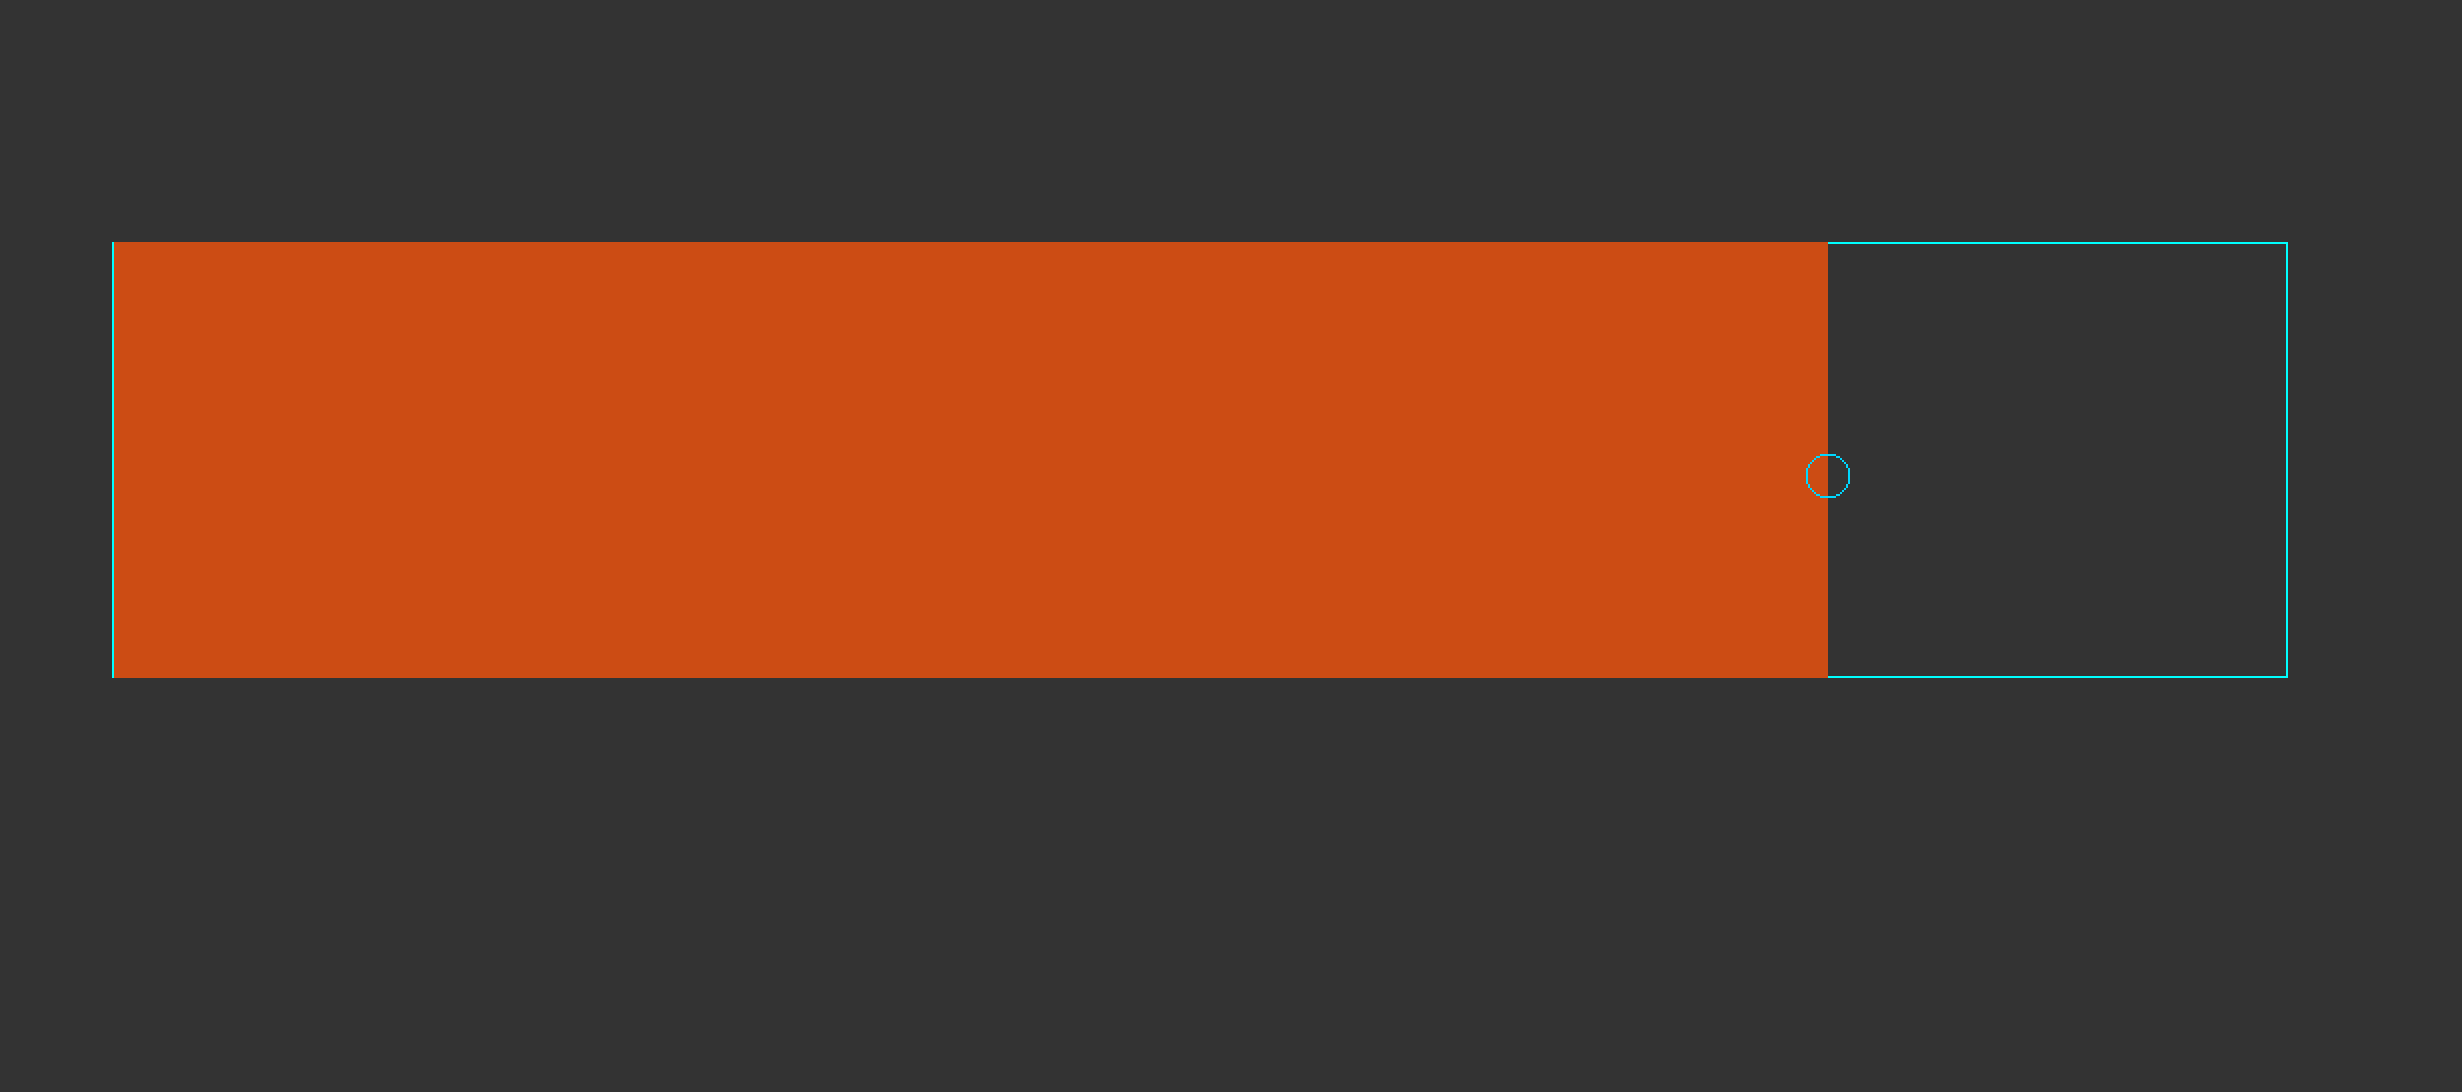
\includegraphics[width=.95\textwidth]{gfx/06_visual_representation/mpTUI_slider-onscreen.png}
			\caption{Rendu du slider dans une fenêtre OpenGL}
		\end{subfigure}%
	}
	\caption{Un simple slider dans la librairie mp.TUI}
\end{figure}

\subsection{Outils pour l'interaction multitouch}

%-------------------------- Figure : mp.TUI overview ------------------------
\begin{figure}[!htbp]
	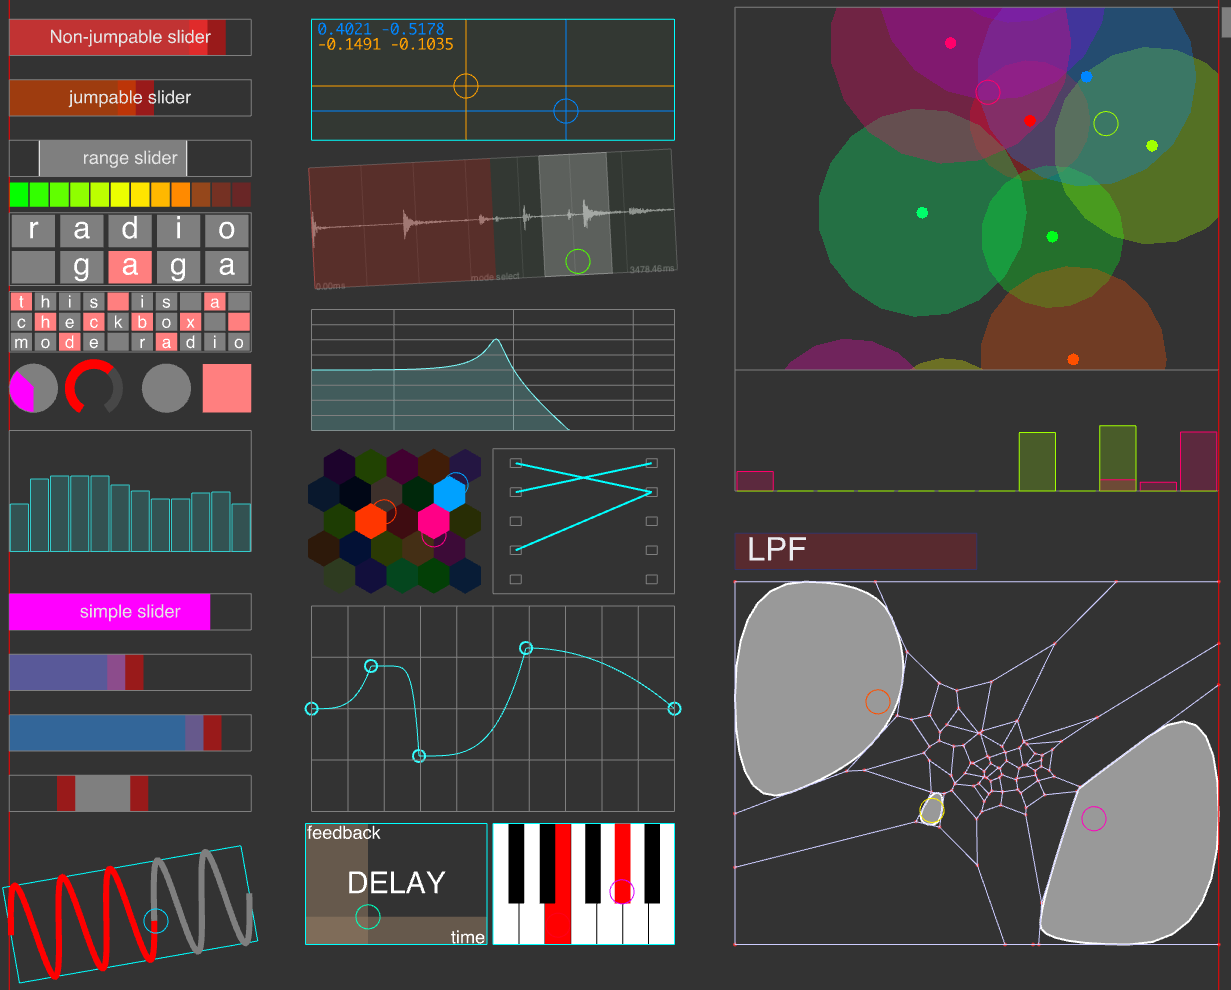
\includegraphics[width=\textwidth]{gfx/mpTUI/mp-TUI-preview.png}
	\caption{Aperçu de quelques composants graphiques de la librairie mp.TUI}
	\label{fig:visual_representation:mp.TUI}
\end{figure}

% \begin{figure}
% 	\captionsetup{format=plain}%
% 	\centering
% 	\begin{minipage}[t]{0.48\textwidth}
% 		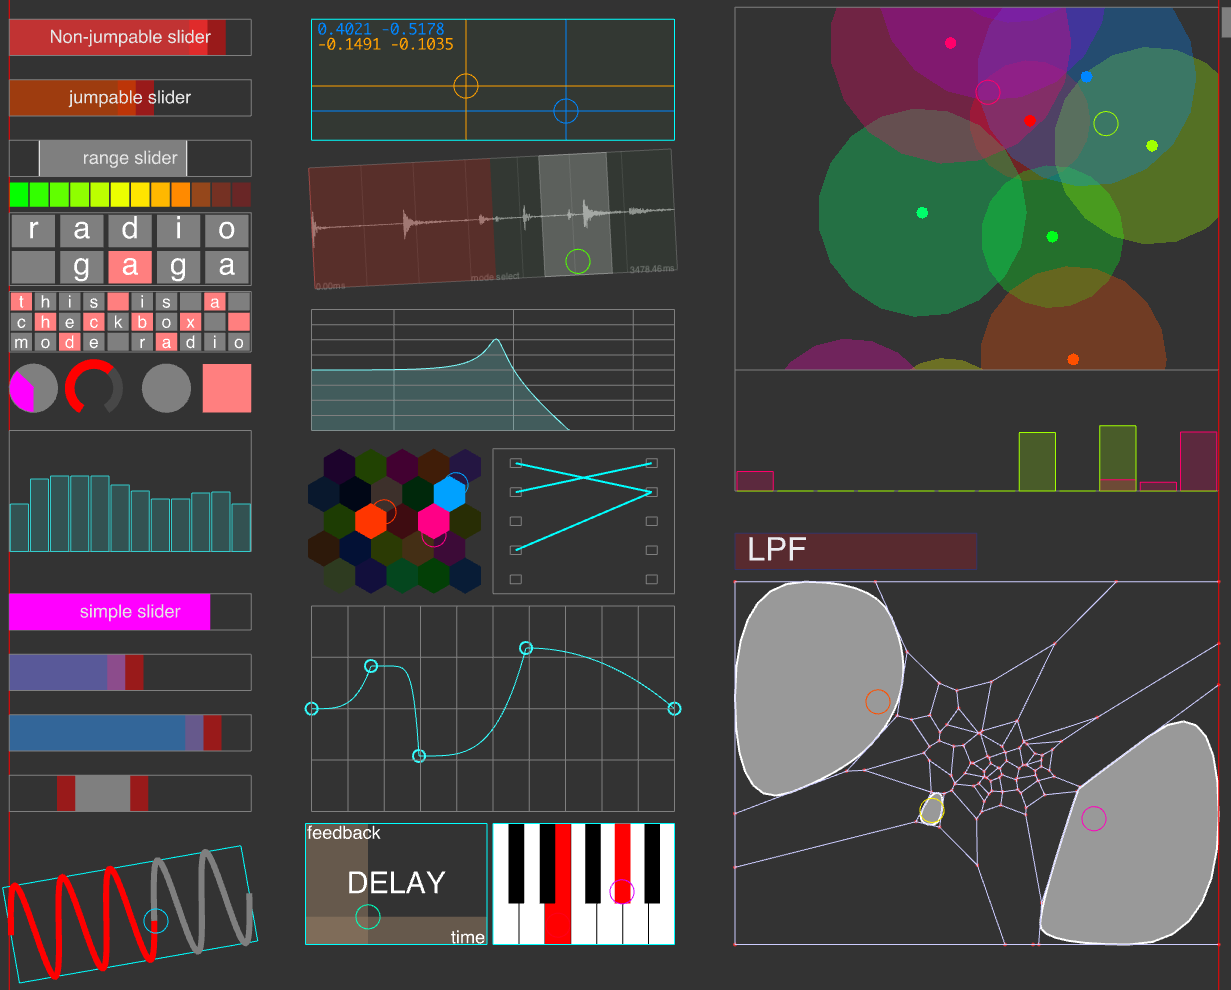
\includegraphics[width=\linewidth]{gfx/mpTUI/mp-TUI-preview.png}
% 		\captionof{figure}{Exemples de composants}	
% 		\label{fig:visual_representation:overview}
% 	\end{minipage}%
% 	\hspace{.02\linewidth}	
% 	\begin{minipage}[t]{0.48\textwidth}
% 	    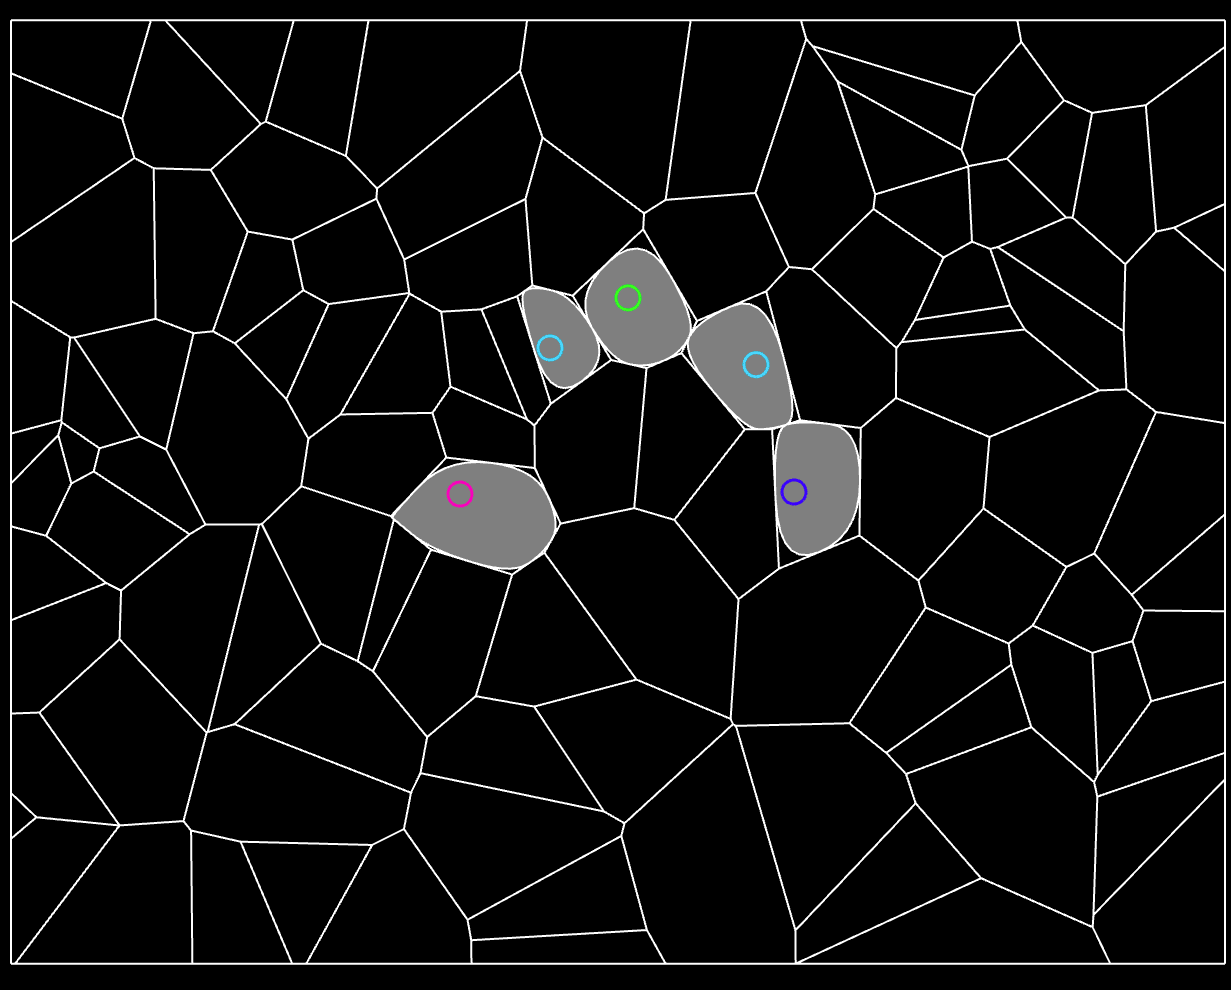
\includegraphics[width=\linewidth]{gfx/mpTUI/mp-TUI-voronoi.png}
% 		\caption{Modèle de Voronoi}
% 		\label{fig:visual_representation:voronoi}
% 	\end{minipage}
% \end{figure}


\subsection{Groupement d'objets graphiques}

\noindent L'objet \verb|mp.TUI.groups| permet de rattacher différents éléments de \gls{GUI} à un groupe, comme on le fait dans la plupart des logiciels d'édition vectorielle, afin de gérer leur position, échelle et orientation de manière globale. Cela permet de définir un ensemble de composants dans des coordonnées relatives, puis de venir ajuster l'emplacement d'un seul et unique bloc. Il est possible de procéder à l'ajustement de ces coordonnées par des valeurs passées explicitement au composant, ou bien par une manipulation directe du groupe, selon le même mode opératoire que pour les objets usuels.\\
\indent Un exemple est présenté sur la figure \ref{fig:visual_representation:groups_patch} et son rendu graphique figure \ref{fig:visual_representation:groups}.

%-------------------------- Figure : groups ----------------------
\begin{figure}[!htbp]
	\captionsetup{format=plain}%
	\centering
	\begin{minipage}[t]{0.48\textwidth}
		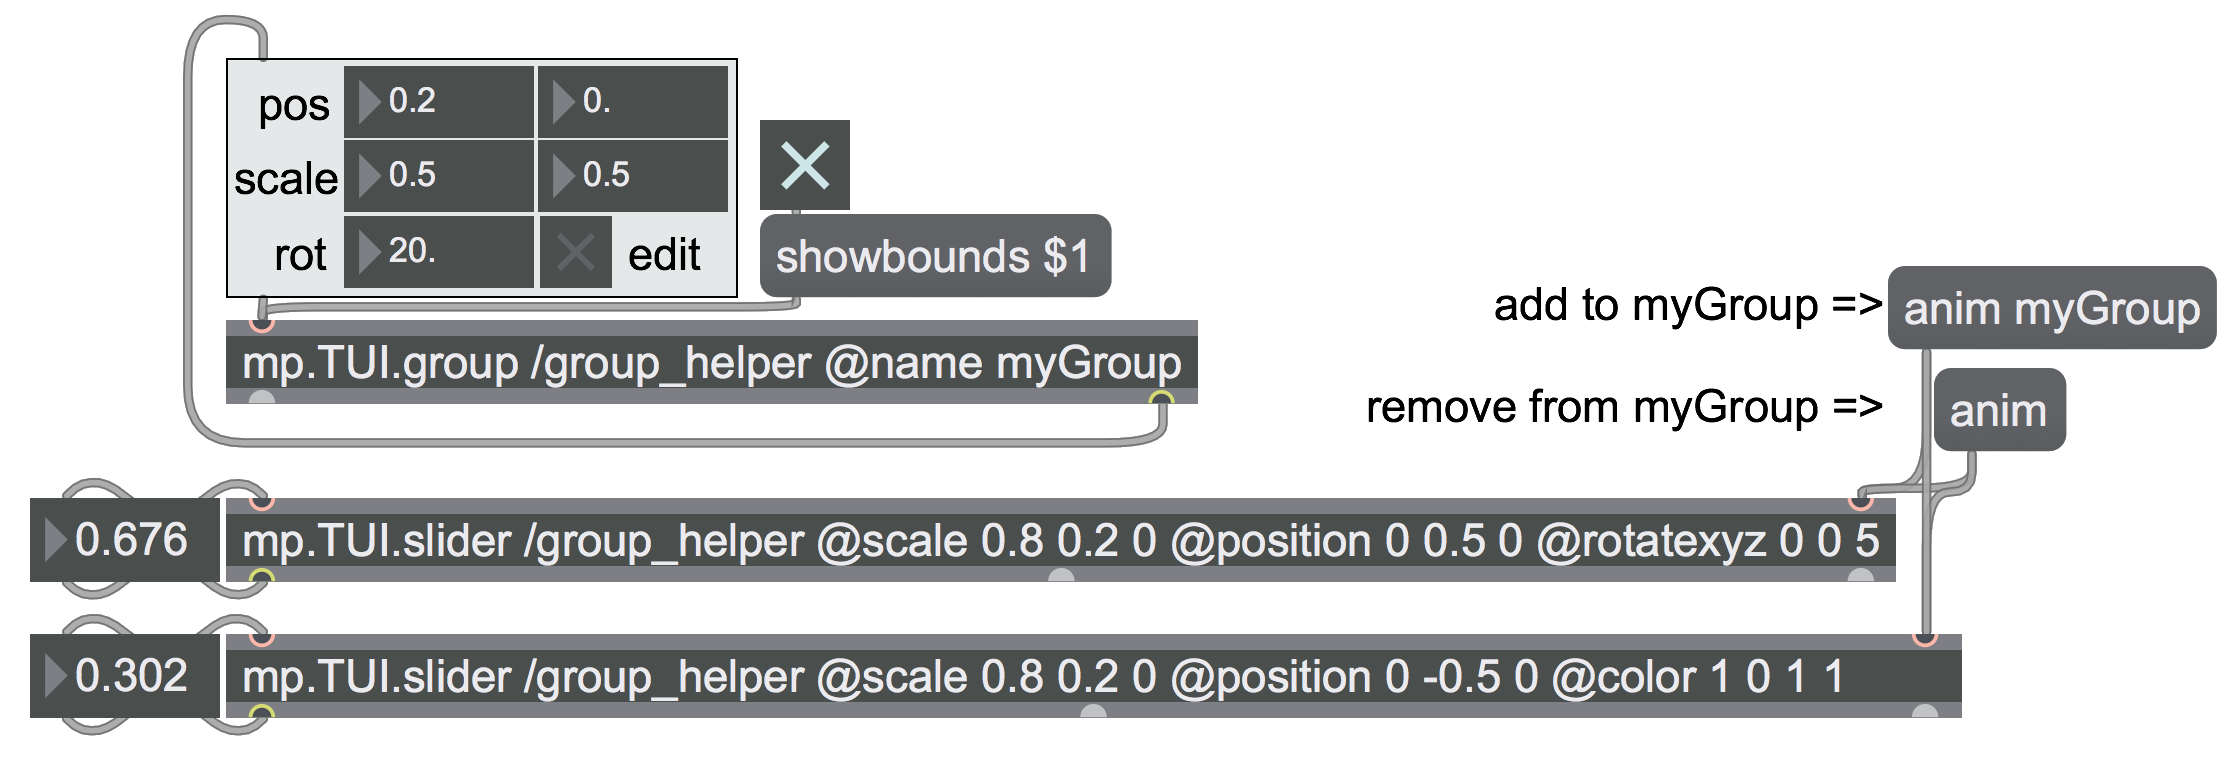
\includegraphics[width=\linewidth]{gfx/06_visual_representation/mpTUI_groups_patcher.png}
		\caption{Patch Max implémentant un groupement de composants mp.TUI.}{Patch Max implémentant un groupement de composants mp.TUI.}
		\label{fig:visual_representation:groups_patch}
	\end{minipage}
	\hspace{.02\linewidth}
	\begin{minipage}[t]{0.48\textwidth}
	    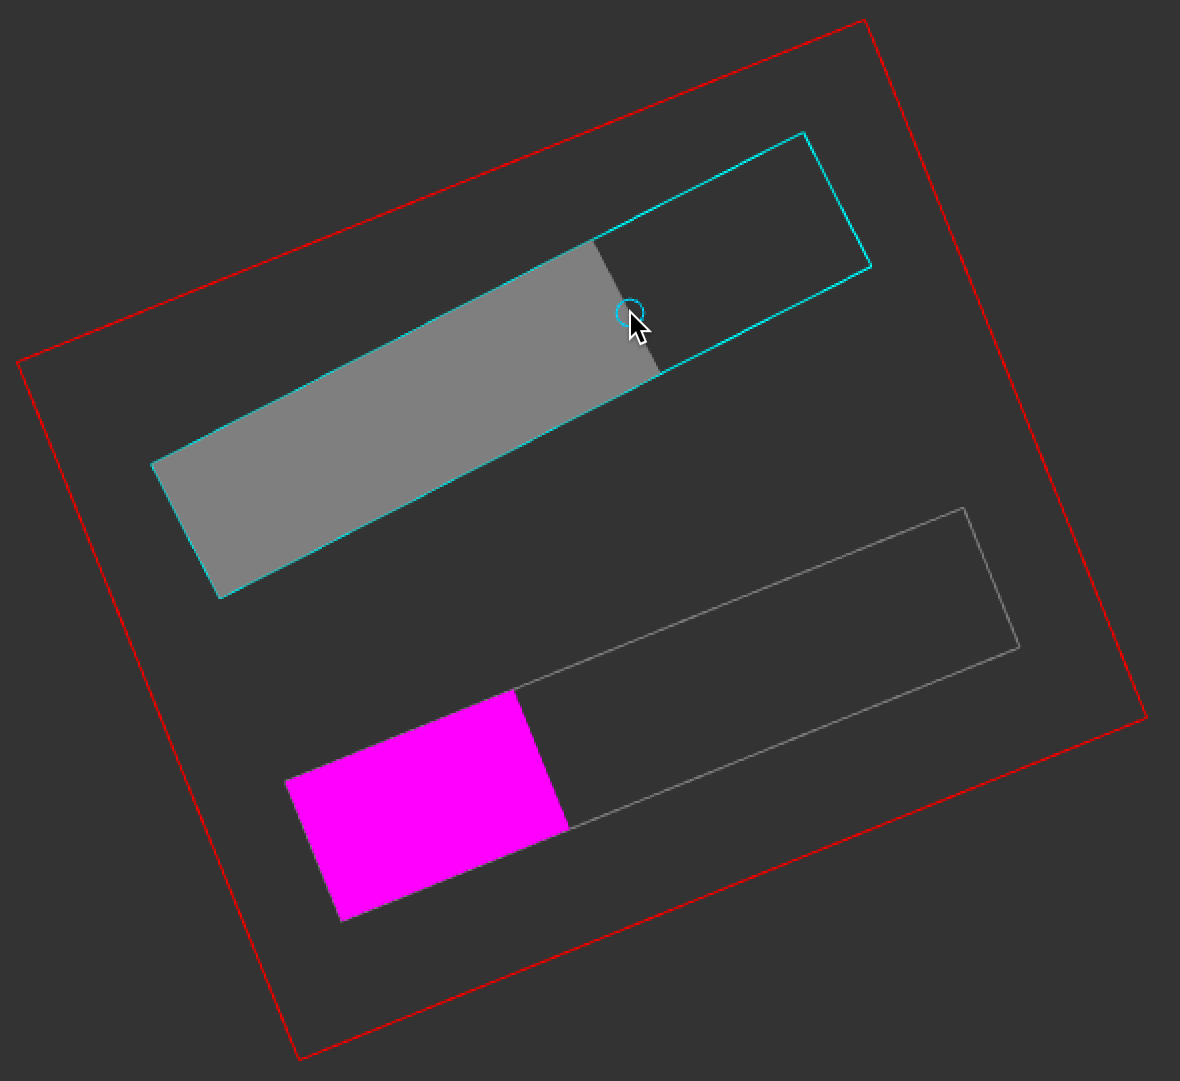
\includegraphics[width=\linewidth]{gfx/06_visual_representation/mpTUI_groups.png}
		\caption[Composants mp.TUI groupés]{Composants groupés et édition ``à la main''. Le cadre du groupe est représenté en rouge.}
		\label{fig:visual_representation:groups}
	\end{minipage}
\end{figure}
%-------------------------- Figure : groups ----------------------

\subsection{GUI composites}

\noindent Il peut s'avérer nécessaire de coordonner plusieurs éléments d'interaction graphique dans un seul et même ensemble, afin qu'un élément puisse réagir à une interaction sur un autre élément. L'objet \verb|mp.TUI.canvas| est destiné à cette fin. C'est un objet graphique vide, qui définit simplement une zone ajustable en position, échelle et orientation. Comme tous les autres objets de la librairie mp.TUI, il émet en sortie les \textit{MP-events} qui lui arrivent, ce qui permet de les renvoyer sur les entrées d'autres composants, même si ceux-ci ne sont pas directement touchés par les curseurs de position.\\
\indent Un exemple simple de \gls{GUI} composite est présenté sur la figure \ref{fig:visual_representation:canvas}, associant des curseurs et un texte affichant leurs coordonnées dans une zone précise définie par le \textit{canvas}.


%------------------ Figure : canvas ---------------------
\begin{figure}[!htbp]
	\captionsetup{format=plain}%
	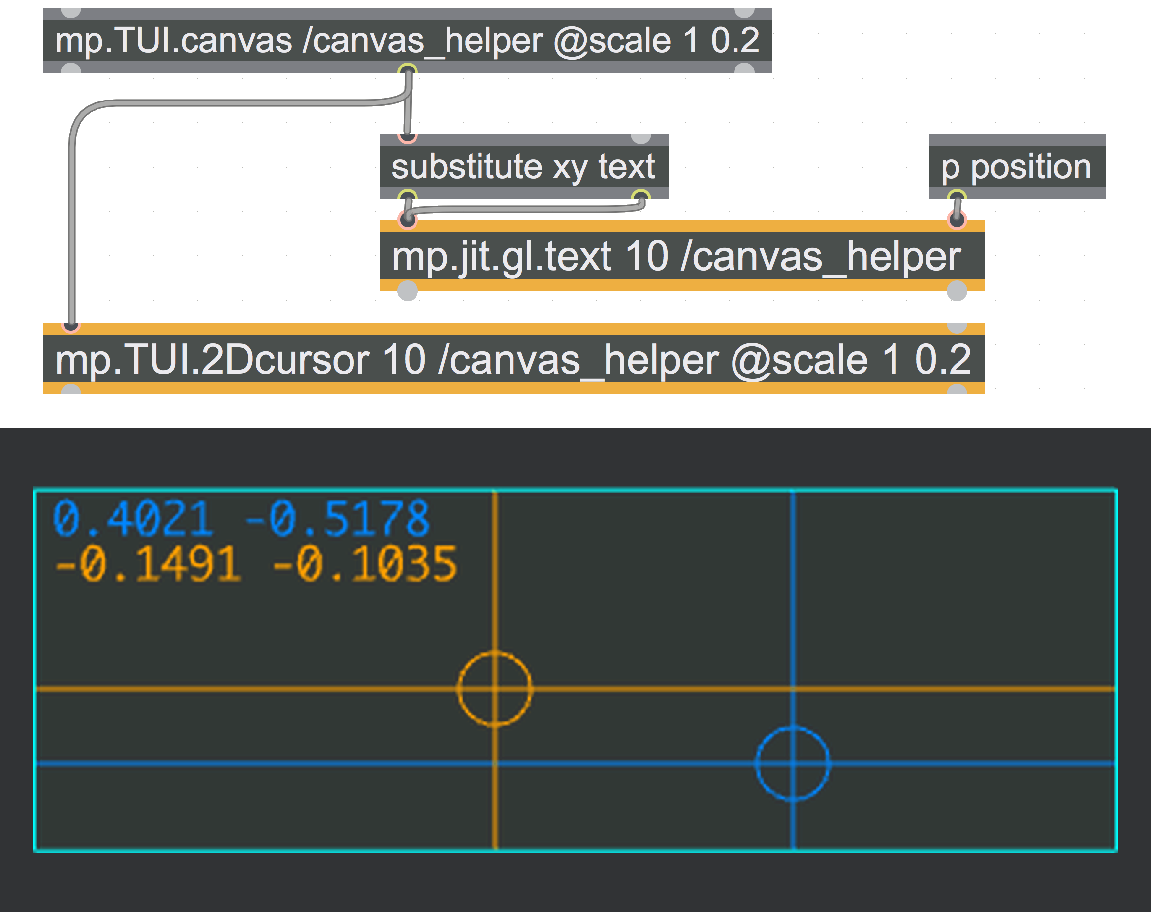
\includegraphics[width=\textwidth]{gfx/06_visual_representation/mpTUI_canvas.pdf}
	\caption[Exemple de GUI composite avec mp.TUI.canvas]{Exemple de GUI composite avec mp.TUI.canvas: les curseurs ne sont pris en compte que dans la zone définie par le \textit{canvas}. Patch Max en haut, rendu en bas.}
	\label{fig:visual_representation:canvas}
\end{figure}
%------------------ Figure : canvas ---------------------

%------------------ Figure : canvas ---------------------
% \begin{figure}[!htbp]
% 	\captionsetup{format=plain}%
% 	\centering
% 	\begin{minipage}[t]{0.38\textwidth}
% 		\includegraphics[width=\linewidth]{gfx/06_visual_representation/mpTUI_composition-canvas.png}
% 		\caption[Exemple de GUI composite avec mp.TUI.canvas]{Exemple de GUI composite avec mp.TUI.canvas}
% 		\label{fig:visual_representation:canvas-patch}
% 	\end{minipage}
% 	\hspace{.01\linewidth}
% 	\begin{minipage}[t]{0.58\textwidth}
% 	  	\includegraphics[width=\linewidth]{gfx/06_visual_representation/mpTUI_canvas_window.png}
% 		\caption[Exemple de GUI composite : rendu graphique]{Exemple de GUI composite : rendu graphique}
% 		\label{fig:visual_representation:canvas-window}
% 	\end{minipage}
% \end{figure}
%------------------ Figure : canvas ---------------------


\subsection{Instanciations dynamiques}

\noindent La gestion de processus musicaux en parallèle créés à la volée nécessite l'instanciation dynamique d'objets, matérialisant de manière tangible ces processus afin de pouvoir les contrôler durant leur existence et les supprimer lorsqu'on le souhaite. Il est parfois possible de poser des objets physiques sur la surface multitouch pour créer et maintenir en vie de tels processus, sans avoir à maintenir le contact des doigts\footnote{C'est le cas par exemple sur la \textit{ReacTable} qui utilise des objets physique cylindriques pour instancier des modules.} (cf. fig \ref{fig:visual_representation:objectOnTable}), mais cette solution n'est pas toujours réalisable\footnote{Les surfaces multitouch basées sur une technologie capacitive ne sont pas sensibles à tous types d'objets physiques, contrairement par exemple, aux écrans basés sur une technologie infra-rouge.} ni souhaitable (pour des raisons d'encombrement de l'espace de la tablette par exemple).\\
\indent Les objets graphiques de la librairie mp.TUI peuvent facilement être créés à la volée pour répondre à ce besoin, en les insérant dans des objets MP, tel que présenté dans le chapitre précédant. Ceci permet de concevoir relativement simplement un scénario d'interaction graphique tel que la possibilité de définir des zones ``réservoir d'objets'' où il est possible de venir piocher des éléments créés dynamiquement, et représentant des processus complexes incluant leur propre mode de destruction (exemple figure \ref{fig:visual_representation:dynamicInstanciation}).
%-------------------------- Figure : maintien curseurs ----------------------
\begin{figure}[!htbp]
	\captionsetup{format=plain}%
	\centering
	\begin{minipage}[t]{0.48\textwidth}
		\includegraphics[width=\linewidth]{gfx/06_visual_representation/mpTUI-stableObject.jpg}
		\caption[Maintien d'un contrôle par un objet physique]{Maintien d'un contrôle par un objet physique. Tout type d'objet sont possible sur une surfac emultitouch par IR; les surfaces capacitives nécessitent des objets conducteurs, voire un circuit électronique dédié et un traitement logiciel \textit{ad-hoc}.}
		\label{fig:visual_representation:objectOnTable}
	\end{minipage}
	\hspace{.02\linewidth}
	\begin{minipage}[t]{0.48\textwidth}
	    \includegraphics[width=\linewidth]{gfx/06_visual_representation/mpTUI-stableObject-dynamic.jpg}
		\caption[Maintien d'un contrôle par un objet virtuel]{Création dynamique de curseurs permettant le maintien d'un contrôle par un objet virtuel. Les curseurs virtuels sont disponibles dans une zone réservoir (drag'n drop) et supprimables, par exemple, par un double clic.}
		\label{fig:visual_representation:dynamicInstanciation}
	\end{minipage}
\end{figure}
%-------------------------- Figure : maintien curseurs ----------------------

\subsection{Performances}

\noindent La bibliothèque mp.TUI est entièrement développée avec des objets natifs de la distribution Max. Cette approche, bien que plus coûteuse en charge \gls{CPU} que des objets compilés, a l'avantage de permettre à tout utilisateur de Max de modifier facilement les composants et de les adapter à ses besoins. De plus, les composants mp.TUI s'appuient essentiellement sur OpenGL, de sorte que la majeure partie de la charge de calcul est laissée au \gls{GPU}, ce qui en fait une solution plus réactive que la solution envisagée dans la libririe MMF. L'interaction tangible avec les objets de la \gls{GUI} se fait à l'aide du moteur physique Bullet-Physics\footnote{\url{http://bulletphysics.org}} intégré dans Max. Bien que cela puisse être plus coûteux pour certaines formes simples, cela nous permet de concevoir des composants \gls{GUI} de n'importe quelle forme et orientation, comme des \textit{sliders} courbes ou des formes évidées, et de les animer avec toutes les possibilités offertes par une modèle physique : champ de forces animant des ensembles d'objets, collisions entre composants, articulations selon des liaisons mécaniques, déplacements inertiels, etc.

\subsection{Travaux futurs}

\noindent Des optimisations sont très probablement possibles pour améliorer les performances de mp.TUI, notamment au niveau du calcul de l'intersection entre position des pointeurs et objets graphiques, en traitant les cas simples séparément plutôt que de les traiter systématiquement dans le modèle générique du moteur \textit{Bullet-Physics}. Cependant, si l'optimisation est toujours utile à la fluidité du rendu graphique, la principale raison d'être de la librairie mp.TUI est le protoypage rapide pour des créateurs non-experts en programmation, et non la finalisation d'une application industrielle pour laquelle des langages plus optimisés (mais plus techniques) offre d'autres solutions.\\
\noindent La librairie mp.TUI permet d'introduire la notion de programmation gestuelle de type \textit{multitouch} dans l'environnement Max, et de bénéficier des possibilités de programmation audio, graphiques et de mapping disponibles, pour les intégrer au fonctionnement des composants de \gls{GUI}. De nombreuses stratégies de contrôle basées sur ce paradigme restent à implémenter, explorer et inventer, notamment sur la gestion d'événements conjoints définissant des primitives gestuelles, tel que présenté dans \cite{oney_implementing_2019}, ou la détection d'objets tagués tels que présenté dans \cite{yu_tuic_2011}. Enfin, le logiciel Max a donné lieu à d'innombrables projets impliquant l'interaction entre le son et l'image, dont les modèles pourraient donner lieu à de nouveaux éléments graphique d'interaction.


\section{Conclusion}

\noindent Nous avions déjà évoqué dans les chapitres précédents la manière dont les \glspl{DMI} intégraient des aspects traditionnellement liés à des domaines différenciés: lutherie traditionnelle, composition, acoustique de l'espace de jeu, psychoacoustique, mais également informatique, et notamment, comme nous l'avons évoqué ici, design graphique.\\
\indent L'infographie se prête à l'hybridation des représentations visuelles liées à ces différents domaines et appelle à leur interaction. Lors de l'usage d'un \gls{DMI}, on peut être amené, par exemple, à ``accorder'' l'acoustique virtuelle d'une salle, selon les fréquences d'une échelle musicale et donc devoir exprimer sous forme de hauteur tonale des paramètres habituellement exprimés en termes de taille de salle, de temps de décroissance, ou de coéfficients de filtres paramétriques. Des représentations visuelles hybrides proposant différentes ``vues'' d'un même modèle peuvent amener à reconsidérer leur usage pour la performance expressive en direct.\\
\indent Un grand nombre de règles de conception graphique ont été édictées depuis le début du \siecle{20}~siècle, visant en particulier à l'efficacité et la clarté des informations qu'elles soutiennent et fréquemment affirmées de manière impérieuse comme des principes à ne pas enfreindre. Pourtant, l'histoire démontre que les innovations dans le domaine de la représentation graphique sont systématiquement survenues lors de la transgression des règles en vigueur, par des artistes imposant un style nouveau (parfois teinté des même préceptes à ne pas enfreindre que leur prédécesseurs)\footnote{Minimalisme fonctionnel du Bauhaus, psychédélisme des années 1970, skeuomorphisme des années 2000, \textit{flat design} de la décade passée, pour ne citer que quelques uns de ces contre-pieds.}.\\
\noindent La représentation visuelle sur les \glspl{DMI} a cela de particulier qu'elle s'inscrit dans un projet artistique où l'importance de la fonctionnalité se partage l'espace visuel avec l'importance de la sensation et de l'évocation poétique. La conjonction de ces deux aspects contribue à ce que la créativité du domaine artistique nourrisse l'innovation dans les aspects fonctionnels de l'instrument.\\
\indent Les représentations visuelles ont précédé de plus de 30.000 ans l'apparition de l'écriture\footnote{On estime actuellement que l'écriture serait apparue il y a environ 5000 ans, en Mésopotamie, tandis que les plus anciennes représentations visuelles datent d'au moins 40.000 ans (peintures rupestres de Borneo et de Blombos), et probablement bien plus (L'âge de la \textit{Venus of Tan-Tan} étant estimée autour de 300.000 ans).} et ont la capacité, plus encore que les symboles alphabétiques, de se superposer, de s'interpénétrer, de recourir à des facteurs d'échelle, des nuances de couleur, de texture, pour communiquer des informations de manière concise et efficace, mais également sensuelle. L'infographie permet d'y ajouter encore une dimension temporelle qui permet toute sorte de métamorphoses et d'hybridation des représentations.\\
\indent Dans ces conditions, le fait de les envisager comme des supports d'interaction laisse présager l'ampleur des possibilités d'invention dans ce domaine. Une spécificité de l'instrument de musique, qui polarise le design graphique dans ce vaste champ des possibles, tient notamment à la disponibilité nécéssaire au musicien pour l'écoute, et lorsque qu'il/elle joue en groupe, l'attention aux autres musicien.nes. C'est en particulier cette écologie de l'attention qui a guidé le développement d'un système de notation musicale sur écran présenté dans le prochain chapitre.



% %%%%%%%%%%%%%%%%%%%%%%%%%%%%%%%%%%%%%%%%%
% \section*{miscellanées (temporaire à supprimer)}


% NIME 2019 : ``From Mondrian to Modular Synth: Rendering NIME using Generative Adversarial Networks''

% Chamagne

% \cite{moody_physics_2009}

% Roel Vertegaal, Tamas Ungvary et Michael Kieslinger utilisait ainsi le terme de ``\textit{musician's cockpit}'' dans un article de 1996, une métaphore qui laisse imaginer l'instrument comme un véhicule que l'on pilote.